\chapter{Grundlagen}\label{grundlagen}

Im folgenden Kapitel werden die Grundlagen beschrieben und erklärt, die für die Erstellung  dieser Masterarbeit benötigt wurden. Zuerst wird die Programmiersprache C++ erklärt und anschließend wird besonders auf die objektorientierte Programmierung eingegangen, die hier als Grundlage dient. Dabei wird zunächst die Grundidee beschrieben. Anschließend wird das Konzept der Klassen und das der Polymorphie dargestellt. Abschließend werden die Grenzen der objektorientierten Programmierung beschrieben.  Weiter wird  die \ac{espdu} des \ac{dis} Protokoll beschrieben. Ein Überblick über die wichtigsten Inhalte des \ac{dis}-Protokoll wird im Grundlagenteil der Studienarbeit \glqq Beurteilung der Open-DIS C++ Library zur Simulation von militärischen Szenarien\grqq{}\cite{HenryWinkel.} der Professur für Technische Informatik an der Helmut Schmidt Univesität der Bundeswehr Hamburg gegeben.


\section{C++ }
C++ ist eine objektorientierte Programmiersprache, die eine Weiterentwicklung der Sprache C ist. Jedoch ist C nicht komplett in C++ enthalten. Bei der Entwicklung von C++ ist man trotzdem dicht an der Syntax von C geblieben. C++ wurde in den 1980er Jahren von Bjarne Stroustrup entwickelt. Für die erste Version, die \glqq C with Classes\grqq{} hieß, versuchte er durch das Nutzen von Teilen der Programmiersprachen Simula und BCPL die Sprache C zu erweitern. Das Konzept der objektorientierten Programmiersprache  wurde aus der Sprache Simula entnommen, die als die erste Programmiersprachen das Klassenkonzept beinhaltet.  BLCP, welche ein Vorgänger von C ist, lieferte den  prozeduralen Anteil.   1983 wurde \glqq C with Classes\grqq{} zu C++ umbenannt. Das erste Release von C++ 1.0 wurde 1985 veröffentlicht. 1998 wurde C++ als Standard \glqq ISO/IEC 14882\grqq{} festgelegt. Im Laufe der Zeit wurde C++ immer weiter verbessert und bekam neue Funktionen. Die aktuellste Version von C++ ist C++17, welches 2017 veröffentlicht wurde.\\
C++ bringt nicht nur eine Reihe von Vereinfachungen und Ergänzungen mit sich, sondern auch diverse Verschärfungen und Änderungen. 
C++ bringt als großen Vorteil die Möglichkeit, objektorientiert zu programmieren. Was genau  \acl{oop} ist, wird in den nachfolgenden Kapitel erklärt. Ein weiterer großer Vorteil von C++ sind Templates. Durch Templates werden unter anderem Container bereitgestellt, die eine dynamische Speicherverwaltung ermöglichen. Container können Listen, Vektoren oder Warteschlagen dynamischer Größe sein, deren Inhalt Elemente einer beliebigen Datenstrukturen sein kann. Neben den Containern, die Klassen-Templates  sind,  gib es noch Funktions-Templates und Variablen-Templates, welche hier nicht weiter erklärt werden, da sie in dieser Masterarbeit keine Anwendung finden. \\
Eine weitere Neuerung in C++ ist die Möglichkeit, Speicher zu reservieren. In C++ kann man durch den Befehl \glqq new\grqq{} Speicher eines beliebigen Typs reservieren. Dieser Befehl ersetzt das \glqq malloc\grqq{} aus C.  Das Gegenstück dazu ist das  \glqq delete\grqq{}. Mit diesem Befehl kann man den reservierten Speicher wieder freigeben. Der Unterschied zwischen  \glqq malloc\grqq{} und \glqq new\grqq{} ist, dass es sich bei \glqq malloc\grqq{} um eine Funktion handelt  und \glqq new\grqq{} ein Operator ist.  Ein weiterer Unterschied  ist, dass \glqq new\grqq{} den Konstruktor einer Klasse aufruft und \glqq malloc\grqq{} dies nicht tut. Weiter muss bei \glqq malloc\grqq{} die zu reservierende Größe des Speichers manuell berechnet werden. Bei  \glqq new\grqq{} wir die Größe vom Compiler bestimmt. \\
In C++ gibt es neben den Pointern auch die Möglichkeit, Referenzen zu benutzen. Der Unterschied zwischen einer Referenz und einem Pointer ist, dass eine Referenz prinzipiell nur eine neue Bezeichnung für eine bereits vorhandene Variable ist.  Neben den genannten Änderungen gibt es noch viele weitere, die jedoch im Rahmen dieser Masterarbeit keine oder nur am Rande benutzt wurden.   
\\
\cite{SebastianMeyer.}
\cite{Krau.}
\cite{Prof.Dr.Ing.WolfgangSchroderPreikschat.}
\cite{HelmutErlenkotter.}
\cite{BenjaminBuch.}
\section{Objektorientiertes Programmieren }

\subsection{Grundidee }
Die Grundidee hinter der objektorientierten Programmierung (\acs{oop}) ist das Abbilden von Objekten der realen Welt. Diese Objekte kommunizieren durch Nachrichten miteinander, welche unterschiedlich interpretiert werden können.  Im Zuge von immer größer werdenden Softwareprojekte hat sich herausgestellt, dass es zum Beispiel mit der Programmiersprache C sehr schwer geworden ist, den  Überblick über den Programmcode und den Programmfluss zu behalten. Objektorientierte Programmiersprachen helfen den Überblick zu behalten und sie bringen Techniken mit sich, Programmteile wieder zu verwenden. Das ermöglicht  das schnellere und fehlerfreiere Entwickeln von Programmen. Ein Nachteil von Programmiersprachen, die ausschließlich objektorientiert sprechen, ist, dass Funktionen nicht alleine existieren können. Dies führt dazu, dass kleine Programme unnötig kompliziert werden. Ein Sprache, die sowohl objektorientiert als auch prozedural verwendet werden kann, ist C++. Wie bereits erwähnt, wird diese Sprache im Rahmen dieser Masterarbeit verwendet.    
Dabei werden unter anderem  Techniken wie die Vererbung und die Polymorphie verwendet. Diese Techniken werden in den folgenden Kapiteln beschrieben. Als Modelierungssprache wurde \ac{uml} und als \ac{ide} wurde Eclipse mit der Papyruserweiterung verwendet. Alle folgenden Beispiele werden anhand dieser Umgebung beschrieben. \\
\cite{HelmutErlenkotter.}
\cite{Prof.Dr.AlfredIrber.}
\cite{Krau.}
\subsection{Klassen und Objekte}
Wie oben genannt, ist die Grundidee hinter der \ac{oop} das Abbilden der realen Welt, um Probleme zu lösen. Ein zentraler Gegenstand hierbei ist die Klasse. Eine Klasse enthält, ähnlich wie das \glqq struct\grqq{} in C, Daten, die Attribute genannt werden. Der Unterschied zu einem klassischen  \glqq struct\grqq{} ist jedoch, dass eine Klasse Funktionen beziehungsweise Methoden enthält, die auf diese Daten zugreifen können. Des Weiteren können  Klassen auch von anderen abgeleitet werden, was Vererbung genannt wird. Die Vererbung wird im nachfolgenden Unterabschnitt erläutert. \\
Um einen unerlaubten Zugriff auf Methoden und Attribute einer Klasse zu verhindern, kann innerhalb der Klasse festgelegt werden, wer auf Inhalte der Klasse zugreifen kann. Dies gliedert sich in drei Gruppen. Funktionen und Methoden können \glqq public\grqq{},  \glqq private\grqq{} oder \glqq protected\grqq{} sein. Soll der Inhalt für jeden zugänglich sein, dann ist er \glqq public\grqq{}. Ist ein Methode oder Attribut \glqq private\grqq{}, dann darf nur von innerhalb der Klasse auf ihn zugegriffen werden. Bei \glqq protected\grqq{} Inhalten können alle von der Klasse abgeleiteten Klassen auf den Inhalt zugreifen.

\begin{figure}[H]
	\centering
	%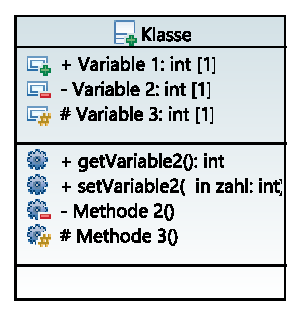
\includegraphics[scale=1.2]{bilder/pdfvorlagen/eineKlasse}
	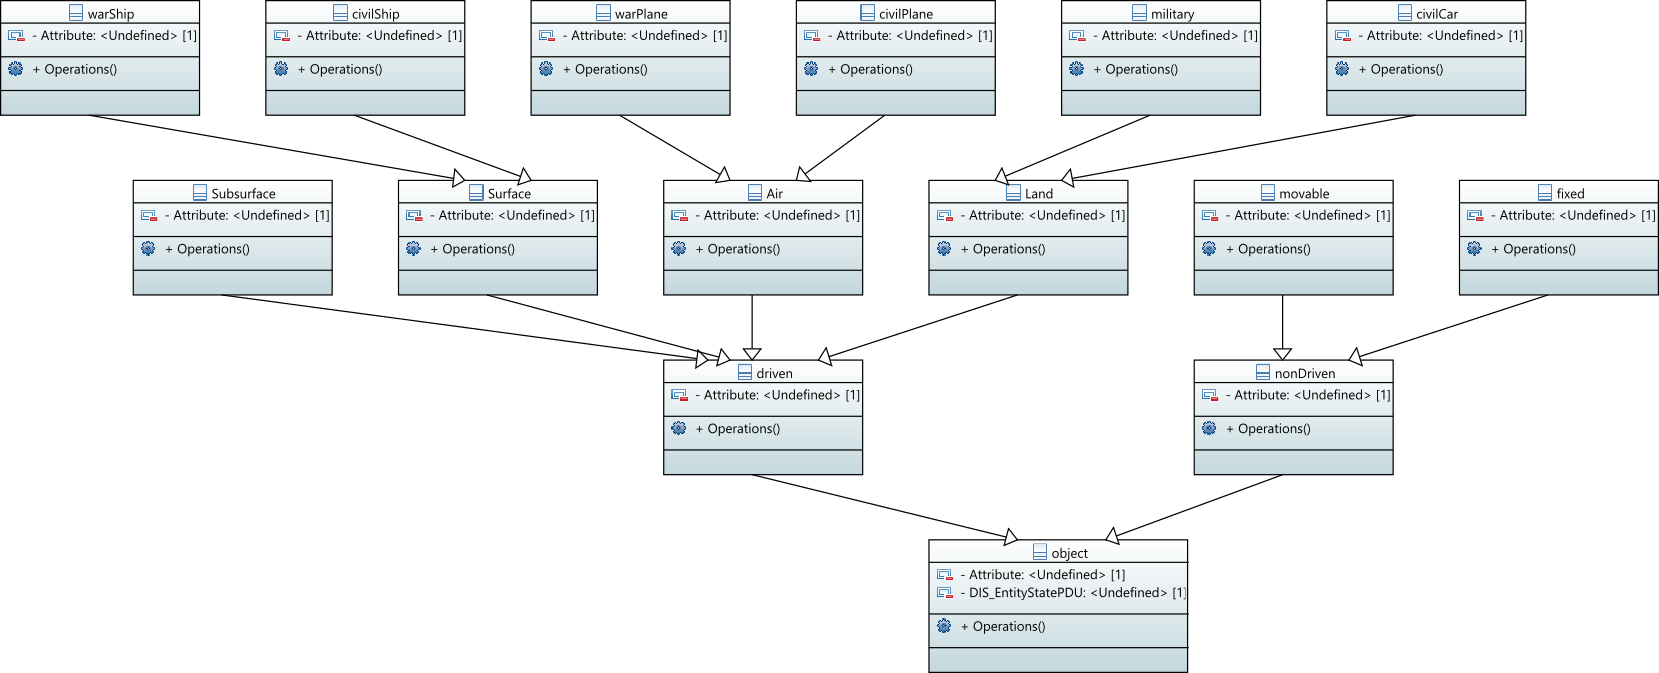
\includegraphics[scale=1]{bilder/pdfvorlagen/model}
	
	\caption[eine Klasse]{eine Klasse}
	\label{fig:eineklasse}
\end{figure}
 In Bild  \ref{fig:eineklasse} ist der exemplarische Entwurf einer Klasse zu sehen. Diese enthält drei Attribute, Variable 1 bis 3, außerdem beinhaltet sie vier Methoden. Ob ein Attribut oder Methode \glqq public\grqq{},  \glqq private\grqq{} oder \glqq protected\grqq{} ist, sieht man an dem Symbol, welches vor dem Namen steht. Das Kästchen mit dem Pluszeichen steht für ein \glqq public\grqq{} Attribut, das Kästchen mit dem roten Balken steht für ein   \glqq private\grqq{} Attribut und das Kästchen mit dem gelben Raute Symbol steht für ein \glqq protected\grqq{} Attribut. Analog gilt das auch für die Methoden, wobei das Pluszeichen bei den \glqq private\grqq{} Methoden entfällt. \\
 Um das unabsichtliche Überschreiben einer Variable zu verhindern, werden in der \acl{oop} Variablen zum Größten Teil als \glqq private\grqq{} deklariert. Wie oben beschrieben, kann die Variable nur innerhalb der eigenen Klasse verändert werden. Um nun die Variable aktiv zu verändern und auszulesen, werden die sogenannten \glqq get\grqq{} und \glqq set\grqq{} Methoden verwendet. Dies sind Methoden, deren Aufgabe es ist, den Zugang zu den Attributen der Klasse zu ermöglichen. Des Weiteren kann mit Hilfe dieser, die korrekte Eingabe überprüft werden. Wie im Bild \ref{fig:eineklasse} zusehen, wurde nur für die Variable zwei eine Methode zum Beschreiben, \glqq setVariable2()\grqq{} und zum Auslesen, \glqq getVariable2()\grqq{}, erstellt.\\
\begin{lstlisting}[caption = Klasse.h,label=klass.h]
#include <iostream>

namespace Beispiel{
class Klasse:{
public:
	int Variable1;
	int getVariable2();
	void setVariable2(int zahl);
protected:
	int Variable;
	void Methode3();
private:
	int Variable2;
	void Methode2();
};
}
\end{lstlisting}
In Listing \ref{klass.h} ist die Header Datei der Beispielklasse aus dem Bild \ref{fig:eineklasse} dargestellt. Hier finden sich alle Methoden und Attribute  wieder. Dabei wird eine Unterteilung nach \glqq public\grqq{},  \glqq private\grqq{} und \glqq protected\grqq{} durchgeführt. In der Header Datei werden nur die Attribute und die Methoden bekannt gegeben. Die Implementation der Methoden findet nicht hier, sondern in einer anderen Datei, der Source Datei, statt.  

 \begin{lstlisting}[caption = Klasse.cpp,label=klass.cpp]
 #include "Klasse1.h"
 
 namespace Beispiel {
 int Klasse1::getVariable2() {
 	return Variable2
 }
  void Klasse1::setVariable2(int zahl) {
  	Variable2 = zahl;
  }
 void Klasse1::Methode2() {
 ...
 }
  
 void Klasse1::Methode3() {
 ...
 }
   
 void Klasse1::Mehtode4() {
 ...
 }
 }
 \end{lstlisting}
 Im Listing \ref{klass.cpp} ist die zum Listing \ref{klass.h} zugehörige Source Datei dargestellt. Wie man sieht, sind hier nur die Implementationen der Mehtoden aufgeführt. Neben den Methoden werden hier auch die statischen Variablen initialisiert. Eine Sortierung, wie in der Header Datei, wird nicht vorgenommen, da  die Zugriffsrechte dort schon festgelegt wurden. 
  \begin{figure}[H]
  	\centering
  	%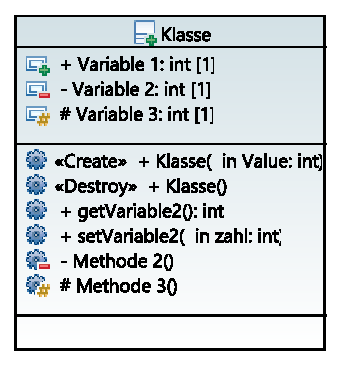
\includegraphics[scale=1.2]{bilder/pdfvorlagen/test2}
  	  	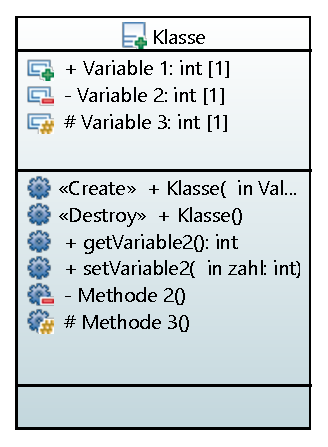
\includegraphics[scale=1.2]{bilder/pdfvorlagen/model2}
  	\caption[eine Klasse mit Konstruktor und Destruktor]{eine Klasse mit Konstruktor und Destruktor}
  	\label{fig:klasseKonstr}
  \end{figure}
Die Klasse stellt jedoch nur den Bauplan für ein Objekt dar. Um die implementierten Methoden zu nutzen, muss man ein Objekt der Klasse erstellt. Dazu kann ein \glqq Konstruktor\grqq{} genutzt werden. Dieser hat den Vorteil, dass die Attribute mit Defaultwerten initialisiert werden können. Der \glqq Konstruktor\grqq{} kann als normale Methode angesehen werden, die jedoch so wie die Klasse benannt sein muss. Er kann deshalb auch Eingabeparameter besitzen und Attribute auf bestimmte Werte setzen. In der \ac{ide} wird als Kennzeichnung für den Konstruktor \glqq Create\grqq{} vor die Methode gesetzt. Möchte man nun das erstellte Objekt wieder löschen, muss man dafür ein  \glqq Destruktor\grqq{} verwenden. Dieser kann ebenfalls als Methode gesehen werden, die den Speicher, der das Objekt belegt, frei gibt. Des Weiteren können im  \glqq Destruktor\grqq{} weitere Anweisungen, wie zum Beispiel das Anpassen eines Zähler, enthalten sein.\\
 Im Bild \ref{fig:klasseKonstr} ist zu sehen, dass der Klasse aus Bild \ref{fig:eineklasse} ein \glqq Konstruktor\grqq{} und \glqq Destruktor\grqq{} hinzugefügt wurden. Diese werden oft als die ersten beiden Methoden angegeben.
  Da die Variablen eines Objektes immer nur so lange existieren, solange wie das Objekt selbst existiert, kann es zum Beispiel keine Variable geben, die Teil der Klasse ist, welche alle erzeugten Objekte zählt. Um dieses Problem zu lösen, kann man auf statische Variablen  zurückgreifen, die auch ohne das erstellte Objekt existieren. Statische Variablen werden unterstrichen, was im Bild \ref{fig:klassestatic} zu sehen ist. Sie können ebenfalls   \glqq private\grqq{}, \glqq public\grqq{} oder  \glqq protected\grqq{} sein und werden auch dementsprechend gleich gekennzeichnet. Neben Attributen können auch Methoden statisch sein. Dies ist ein Vorteil, wenn man nur eine bestimmte Funktion der Klasse benutzen möchte, ohne erst das Objekt zu erstellen und anschließend wieder löschen zu müssen. In Listing \ref{vererbungc++} ist die Header Datei, welche den Konstruktor und den Destruktor enthält, dargestellt. Die Implementierung erfolgt wie bei einer normalen Methode in der Source Datei. 
  \begin{figure}[H]
 	\centering
 	%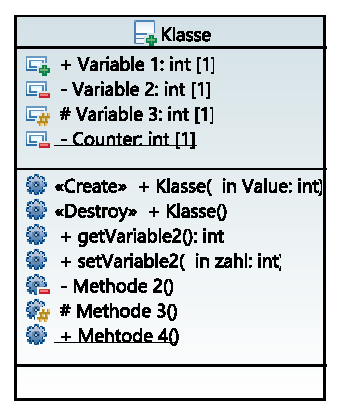
\includegraphics[scale=1.2]{bilder/pdfvorlagen/static}
 	 	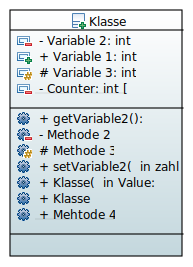
\includegraphics[scale=1.2]{bilder/pdfvorlagen/model3}
 	\caption[eine Klasse mit statischer Variable]{eine Klasse mit statischer Variable}
 	\label{fig:klassestatic}
 \end{figure}
\cite{HelmutErlenkotter.}
\cite{Prof.Dr.AlfredIrber.}
\cite{Krau.}
\subsection{Vererbung}
Ein Vorteil der \ac{oop} ist, dass Klassen von anderen Klassen Attribute und Methoden erben können. Das bedeutet, dass die erbende Klasse Zugriff auf alle \glqq public\grqq{} und  \glqq protected\grqq{} Methoden und Attribute hat. Die erbende Klasse wird Kindklasse genannt und die Klasse, von der geerbt wird, wird Elternklasse genannt. In Bild \ref{fig:vererbung} sind zwei Klassen abgebildet, die Klasse 1 und die Klasse2. Die Klasse1 erbt von Klasse2 alle Attribute und Methoden. In diesem Beispiel erbt Klasse 1 das Attribut   \glqq Name\grqq{} und die Methoden  \glqq setName()\grqq{} und  \glqq getName()\grqq{} von Klasse2. Eine Elternklasse kann mehrere Kinder haben, was bedeutete, dass in Elternklassen Attribute und Methoden beinhaltet sein können, die jede ihrer Kindklassen benötigt. Das reduziert den Aufwand bei der Erstellung der Methoden, da sie nur einmal in den Elternklassen implementiert werden müssen.   
 \begin{figure}[H]
	\centering
	%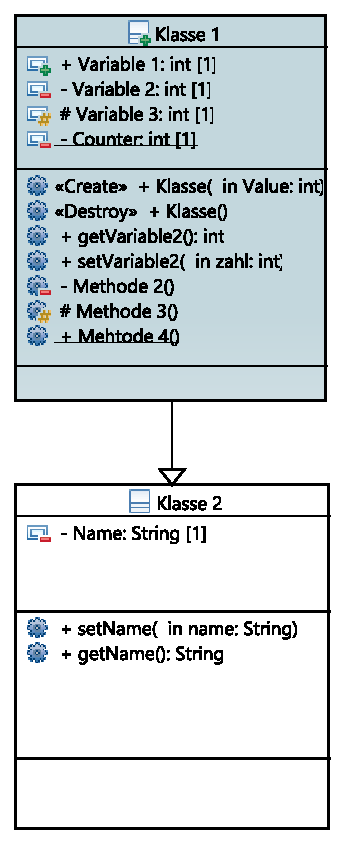
\includegraphics[scale=1]{bilder/pdfvorlagen/vererbung.pdf}
		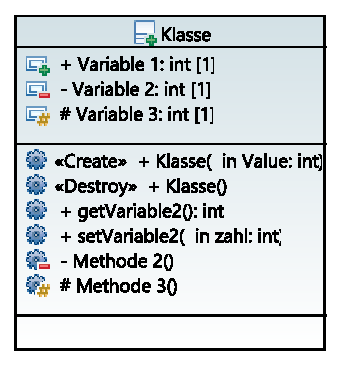
\includegraphics[scale=0.9]{bilder/pdfvorlagen/tes.pdf}
	\caption[Vererbung]{Vererbung}
	\label{fig:vererbung}
\end{figure}
\newpage
In Listing \ref{vererbungc++} ist die Header Datei der Klasse2 dargestellt. Das  \glqq public\grqq{} vor Klasse2 gibt an, wie von dieser Klasse geerbt wird. Die Methoden und Attribute der Elternklasse werden hier nicht angegeben, da diese in der Header Datei der Elternklasse deklariert und in der Source Datei implementiert werden.
\begin{lstlisting}[caption =Vererbung in C++,label=vererbungc++]
#include <iostream>
#include "Klasse2.h"

namespace Beispiel{
class Klasse1: public Klasse2:{
public:
	Klasse1(int Value);
	~Klasse1();
	int Variable1;
	int getVariable2();
	void setVariable2(int zahl);
protected:
	int Variable3;
	void Methode3();
private:
	int Variable2;
	void Methode2();
};
}
\end{lstlisting}
Die oben beschriebene Vererbung ist eine \glqq public\grqq{} Vererbung. Neben dieser Art können Klassen auch \glqq private\grqq{} oder \glqq protected\grqq{} erben. Dies verändert die Zugriffsmöglichkeiten auf die Elemente, also die Methoden und Attribute der Elternklasse.
Ist zum Beispiel eine Methode in der Elternklasse  \glqq public\grqq{} und wird diese durch eine \glqq private\grqq{} Vererbung vererbt, so ist diese Methode in der Kindklasse \glqq private\grqq{} und kann nur innerhalb dieser Klasse benutzt werden.
In Tabelle \ref{vererbungKlassen} sind die verschiedenen Methoden und deren Konsequenzen dargestellt.
\begin{table}[H]
	\centering
	\begin{tabular}{|l|l|l|}
		\hline
		\textbf{Ableitung} & \textbf{Privileg der Elternklasse} & \textbf{Privileg der Kindklasse} \\ \hline
		\textbf{public}   & public                             & public                           \\ \hline
		& protected                          & protected                        \\ \hline
		& private                            & kein Zugriff                     \\ \hline
		\textbf{private}   & public                             & private                          \\ \hline
		& protected                          & private                          \\ \hline
		& private                            & kein Zugriff                     \\ \hline
		\textbf{protected} & public                             & protected                        \\ \hline
		& protected                          & protected                        \\ \hline
		& private                            & kein Zugriff                     \\ \hline
	\end{tabular}
\caption[Vererbung von Klassen]{Vererbung von Klassen}
\label{vererbungKlassen}
\end{table}
In Listing \ref{use} ist in Zeile 5  zusehen, wie man mithilfe eines Konstruktors, ein Objekt von Typ Klasse1 erstellt. In Zeile 6 wird eine Methode aus der eigenen Klasse benutzt. Dazu wird hinter den Namen des Objektes, hier \glqq Klasse1\grqq{}, der Aufruf der Methode gesetzt. Der Aufruf einer Methode aus der Elternklasse erfolgt wie der Aufruf einer Methode der eigenen Klasse. Dies ist in Zeile 7 zusehen. Abschließend wird das Objekt durch den Destruktor, in Zeile 8 zusehen, gelöscht. 
\begin{lstlisting}[caption = Benutzung der Klasse,label=use]
#include <iostream>
#include "Klasse1.h"

int main(){
Beipiel::Klasse1 Klasse1(1);
Klasse1.setVariable2(2);
Klasse1.getName();
Klasse1.~Klasse1();
return 0;
}
\end{lstlisting}
\cite{HelmutErlenkotter.}
\cite{Prof.Dr.AlfredIrber.}
\cite{Krau.}
\subsection{Polymorphie}\label{poly}
Neben der Vererbung ist die Polymorphie ein weiteres Grundkonzept der \ac{oop}. Polymorphie ermöglicht verwandte Objekte mithilfe gleichnamiger Funktionsaufrufe zu verarbeiten. Bevor jedoch die Polymorphie ausführlich erklärt werden kann, müssen zunächst einige Voraussetzungen erklärt werden.
Zu diesen gehört das Umwandeln von Klassen. Für das Umwandeln von  Klassen beziehungsweise von Objekten, gibt es mehrere Möglichkeiten. Die Erste ist die direkte Zuweisung. Dabei muss man beachten, dass dies nur in eine Richtung funktioniert. Das heißt, dass nur Objekte einer Kindklasse in ein Objekt einer Elternklasse umgewandelt werden kann. Der Grund dafür ist, dass jedes Attribut der Ziel Klasse belegt werden muss und dabei gehen die eigenen  Attribute und Methoden  der Kindklasse verloren.\\
Eine weitere Methode ist das Umwandeln mithilfe eines Pointers.
Dazu wird zunächst ein Pointer erstellt, der auf ein Objekt der Elternklasse zeigt. Diesen Zeiger kann die Speicheradresse eines Objektes der Kindklasse übergeben werden. Über diesen Zeiger kann nun auf Methoden zugegriffen werden, die in der Elternklasse enthalten sind. Auf die Methoden der Kindklasse kann nicht zugegriffen werden. Die Umwandlung mittels Pointern ermöglicht, im Gegensatz zur Umwandlung durch Zuweisung, eine Konvertierung eines Objektes der Elternklasse in ein Objekt der Kindklasse. Dabei muss jedoch zwingend ein \glqq stativ\_cast\grqq{} auf das Objekt angewendet werden, welches umgewandelt werden soll. \\
Das Umwandeln von Klassen ermöglicht es, Objekte unterschiedlicher Klassen gemeinsam zu verarbeiten. 
Um nach dem Umwandeln eines Objektes auch auf die dazugehörige Methode zugreifen zu können, muss die Elternklasse, in die das Objekt umgewandelt werden soll, virtuelle Funktionen besitzen. 
\newpage
\begin{lstlisting}[caption = Klasse2.h,label=parent]
#include <iostream>

namespace Beispiel{
class Klasse2 {
public:
	void setName(std::string name);
	std::string getName();
	virtual void printName();
private:
	std::string Name;
};
}
\end{lstlisting}
In Listing  \ref{parent} ist die Header Datei der Elternklasse zu sehen. Diese verfügt über die virtuelle Methode \glqq virtual void printName()\grqq{}. Das 
\glqq virtuel\grqq{} vor dem Funktionsaufruf sorgt dafür, dass diese Methode in allen Kindklassen implementiert werden muss. In der Kindklasse tauchte diese Mehtode als ganz normale Methode auf, dabei muss sie den gleichen Namen wie die virtuelle Methode aus der Elternklasse haben.\\
In Listing \ref{virtuel} wird gezeigt, wie man ein Objekt der Kindklasse mithilfe eines Pointers in ein Objekt der Elternklasse umwandelt. Dabei wird in Zeile 5  zunächst ein Pointer erzeugt, der auf ein Objekt der Klasse2 zeigt. Diesem Pointer wird anschließend in Zeile 7 die Speicheradresse des Objektes der Klasse1 übergeben. Der Klasse1 wird nun mittels Funktionsaufruf der Name  \glqq hallo welt\grqq{} zugeordnet. Im Anschluss wird durch die Ausgabe überprüft, ob der Name dem Objekt zugeordnet wurde. Dies ist in Zeile 9 zu sehen. In Zeile 10 ist zu sehen, wie mit Hilfe des Zuweisungsoperators \glqq ->\grqq{} die Fuknktion \glqq printName()\grqq{}, der Elternfunktion, aufgerufen wird. Da es kein Objekt der Elternklasse gibt, könnte man jetzt meinen, dass dieser Aufruf einen Fehler erzeugen würde. Aufgrund der aufgerufenen virtuelle Methode, wird nun nicht die Mehtode der Elternklasse ausgeführt. Da das Objekt, auf das der Pointer zeigt, ein Objekt der Kindklasse ist, wird nun entschieden, dass es die Implementation aus der Kindklasse verwendet. Diese Entscheidung erfolgt automatisch während der Laufzeit. \\
Wie erwartet, gibt das Programm zwei mal hintereinander \glqq hallo welt\grqq{} aus. Das erste Mal kommt von dem \glqq std::cout << Klasse1.getName() << std::endl;\grqq{} und das zweite Mal kommt entsprechend von dem \glqq Klasse2->printName();\grqq{}.
\begin{lstlisting}[caption = Beispiel virtuelle Funktion,label=virtuel]
#include <iostream>

int main() {
tes::Klasse1 Klasse1(2);
tes::Klasse2 *Klasse2;

Klasse2 = &Klasse1;
Klasse1.setName("hallo welt");
std::cout << Klasse1.getName() << std::endl;
Klasse2->printName();
Klasse1.~Klasse1();

return 0;
}
\end{lstlisting}
Virtuelle Methoden müssen  auch eine Implementierung in der Elternklasse besitzen. Um dies zu umgehen, kann eine Methode \glqq pure virtual\grqq{} sein. Dazu setzt man in der Header Datei die virtuelle Methode gleich 0. Dies hat zur Konsequenz, dass die gesamte Klasse abstrakt wird. Von abstrakten Klassen können keine Objekte erzeugt werden. 
\\
Neben den genannten Inhalten der Polymorphie gib es noch weitere, wie zum Beispiel die virtuellen Destruktoren oder die Möglichkeit, sich den Objekttyp ausgeben zu lassen. Diese Inhalte wurden in dieser Masterarbeit nicht benutzt und werden daher nicht weiter betrachtet.
\\
Die Polymorphie beschreibt also, wie man mit Objekten verwandter Klassen umgehen kann und wie diese auf einfache Weise verwaltet werden können, ohne dass der Anwender zu jeder Zeit weiß, welche Methode er für welches Objekt benutzt muss. Diese Entscheidung wird ihm von Programm selbst abgenommen. 
\\
\cite{HelmutErlenkotter.}
\cite{Prof.Dr.AlfredIrber.}
\cite{Krau.}

\section{\acl{dis}}
\acf{dis} steht für einen Standard zur Steuerung und Überwachung  von Simulationen, der 1993 im \ac{ieee} 1278 definiert wurde. Er wird für Simulationen im militärische und zivilen Umfeld genutzt und ermöglicht das Erstellen und das Vernetzten von Simulationen sowie das Erstellen von simulierten Lagebildern. Dabei können die einzelnen Simulationen unterschiedliche Sprachen sprechen. Genauere Informationen über den Aufbau und die Inhalte von \ac{dis} können in der Studienarbeit \glqq Beurteilung der Open-DIS C++ Library zur Simulation von militärischen Szenarien\grqq{} und im \ac{dis} Standard nachgelesen werden. Die verwendete Library ist wie in der aufgeführten Studienarbeit die  \glqq Open-DIS\grqq{} Library. Da im Rahmen dieser Masterarbeit ausschließlich mit der \acf{espdu} gearbeitet wurde, wird diese im kommenden Abschnitt vertieft erklärt.\\
Die \ac{espdu} ist eines der Grundelemente von \ac{dis}. Mit ihrer Hilfe werden Entitäten dargestellt, welche für bestimmte Objekte wie Panzer, Schiffe oder Fahrzeuge stehen. Die \ac{espdu} stellt eine Klasse dar, die folgende Attribute besitzt:
\begin{itemize}
	\singlespacing
	\item \ac{pdu} Header
	\item Entity ID
	\item Force ID
	\item Number of Variable Parameter Records(N)
	\item Entity Type
	\item Alternative Entity Type
	\item Entity Linear Velocity
	\item Entity Location
	\item Entity Orientation
	\item Entity Appearance
	\item Dead Reckoning Parameters
	\item Entity Marking
	\item Capabilities
	\item Variable Parameter record \#1
	\item Variable Parameter record \#N
\end{itemize} 


\begin{table}[H]
	\centering
	\begin{tabular}{|l|c|l|}
		\hline
		\multicolumn{1}{|c|}{Field size} & \multicolumn{2}{l|}{Entity State PDU field}    \\ \hline
		\multirow{8}{*}{96 bits}        & \multirow{8}{*}{PDU Header} & Protocol Version \\ \cline{3-3} 
		&                             & Exercise ID      \\ \cline{3-3} 
		&                             & PDU Type         \\ \cline{3-3} 
		&                             & Protocol Family  \\ \cline{3-3} 
		&                             & Timestamp        \\ \cline{3-3} 
		&                             & Length           \\ \cline{3-3} 
		&                             & PDU Status       \\ \cline{3-3} 
		&                             & Padding          \\ \hline
	\end{tabular}
\caption[\ac{pdu} Header]{\ac{pdu} Header\cite{SISOStandardsActivityCommitteeoftheIEEEComputerSociety.}}
\label{header}
\end{table}
Der \ac{pdu} Header beinhaltet die grundlegenden Informationen über die \ac{pdu} und die Simulation. Dabei sollten die Werte für die \glqq Protocol Version\grqq{} und der \glqq Exercise ID\grqq{} bei allen Teilnehmern der Simulation gleich sein. Dies zeigt zum einen die verwendete \ac{dis} Version und die Simulationsnummer einer spezifischen Simulation.   


\begin{table}[H]
	\begin{tabular}{|c|l|l|}
		\hline
		Field size             & \multicolumn{2}{l|}{Entity State PDU field}                  \\ \hline
		\multirow{3}{*}{48 bits}    & \multirow{3}{*}{Entity ID}              & Site Number        \\ \cline{3-3} 
		&                                         & Application Number \\ \cline{3-3} 
		&                                         & Entity Number      \\ \hline
		8 bits                      & Force ID                                & enumeration        \\ \hline
		8 bits                     & Number of Variable Parameter Records(N) & unsigned integer   \\ \hline
	
	\end{tabular}
\caption[Entity ID, Force ID und anzahl Parameter]{Entity ID, Force ID und anzahl Parameter\cite{SISOStandardsActivityCommitteeoftheIEEEComputerSociety.}}
\label{ids}
\end{table}
In Tabelle \ref{ids} ist angeben, wie sich der Inhalt der Entity ID zusammensetzt.
Die Werte hängen dabei von einander ab. Die  \glqq Site Number\grqq{} gibt Auskunft darüber, an welchem geografischen Ort die Simulation stattfindet.
Die \glqq Application Number\grqq{} gibt an, welche Anwendung die \ac{espdu} Simuliert hat. Die \glqq Entity Number\grqq{} gibt an, ob es sich bei der \ac{espdu} um eine befreundete, feindliche, neutrale oder um eine Einheit anderer Gesinnung handelt. Des Weiteren kann aus ihr entnommen werden, die wievielte Einheit es ist. Die \glqq Entity Number\grqq{} hängt dabei von der \glqq Site Number\grqq{} ab. Bei einer anderen \glqq Site Number\grqq{} kann die sonst einmalige \glqq Entity Number\grqq{} erneut vergeben werden. Die \glqq ForceID\grqq{} gibt die eindeutige Nummer der Entity an und \glqq Number of Variable Parameter Records(N)\grqq{} gibt die Anzahl der Zusatzparameter an. Diese werden im weiteren Verlauf ausführlich erklärt. 


\begin{table}[H]
	\centering
	\begin{tabular}{|c|c|l|}
		\hline
		Field size               & \multicolumn{2}{c|}{Entity Sate PDU fields} \\ \hline
		\multirow{7}{*}{64 bits} & \multirow{7}{*}{Entity Type}  & Entity Kind \\ \cline{3-3} 
		&                               & Domain      \\ \cline{3-3} 
		&                               & Country     \\ \cline{3-3} 
		&                               & Category    \\ \cline{3-3} 
		&                               & Subcategory \\ \cline{3-3} 
		&                               & Specific    \\ \cline{3-3} 
		&                               & Extra       \\ \hline
	\end{tabular}
\caption[Entity Type ]{Entity Type\cite{SISOStandardsActivityCommitteeoftheIEEEComputerSociety.}}
\label{type}

\end{table}
Der Entity Type gibt Auskunft darüber, um was für eine spezielle Art es sich bei der \ac{espdu} handelt und welcher Nation diese angehört. Der Inhalt des Entity Type wird durch die \ac{dis} Enumeration begrenzt. In der Enumeration werden militärische Fahrzeuge wie Flugzeuge, Schiffe, Boote und Landfahrzeuge, verschiedener Nationen kodiert. Ein alternativer Entity Type kann im Feld \glqq Alternative Entity Type\grqq{} angeben werden.\\
Die  \glqq Entity Linear Velocity\grqq{}, \glqq Entity Location\grqq{} und \glqq Entity Orientation\grqq{} sind  dreidimensionale Vektoren. Der  \glqq Entity Linear Velocity\grqq{} Vektor gibt die vektorielle Geschwindigkeit, der \glqq Entity Location\grqq{} Vektor die Position und der \glqq Entity Orientation\grqq{} Vektor die Orientierung an. \\
Das  \glqq Entity Appearance\grqq{} Feld ist ein 32 Bit breiter Vektor, welcher Informationen über die Gesamterscheinung der \ac{espdu} angibt. Beispielsweise kann in diesem Vektor kodiert sein, welche Lackierung die Entity hat, ob die Entity beschädigt ist oder ob sie sich selbstständig bewegen kann. Genauere Informationen sind in der \ac{dis} Enumeration beschrieben.\\
 Die  \glqq Dead Reckoning Parameters\grqq{}  geben an, welche Methode verwendet werden muss, um die Position der Entity vorauszuberechnen. Dieses Feld dient zur Reduzierung der Netzwerkauslastung.\\
 Das \glqq Entity Marking\grqq{} Feld enthält Informationen über eindeutige Markierungen an der Entity. Dies können zum Beispiel Zahlen, Symbole oder Ländersymbole sein.\\ Das \glqq Capabilities\grqq{} ist ein 32 Bit breiter Vektor, welcher angibt, welche Fähigkeiten eine Entity besitzt. Zu Diesen  gehört Beispielweise die 
Fähigkeit, andere Entity's mit Munition oder Treibstoff zu versorgen. Ausführliche Informationen sind in der \ac{dis} Enumeration enthalten.

\begin{table}[H]
	\centering
	\begin{tabular}{|l|l|l|}
		\hline
		Field size                & \multicolumn{2}{l|}{Entity State PDU fields}                        \\ \hline
		\multirow{2}{*}{128 bits} & \multirow{2}{*}{Variable Parameter record} & Record Type            \\ \cline{3-3} 
		&                                            & Record-Specific fields \\ \hline
	\end{tabular}
\caption[Variable Parameter record ]{Variable Paramete record\cite{SISOStandardsActivityCommitteeoftheIEEEComputerSociety.}}
\label{variable}
\end{table}
Im Variable Parameter record werden die Zusatzteile beschrieben, die an dem \ac{espdu} verbaut sind. Dazu können Waffenanlagen und Sensoranlagen gehören. In Tabelle \ref{variableex} ist ein Turm mit Kanone als  Variable Parameter record in \ac{dis} dargestellt. Da sich der Turm drehen und die Kanone sich anheben können soll, werden vier Parameter benötigt, die die Bewegung beschreiben. Dabei gibt es einen Parameter Record, der die aktuelle Lage beschreibt. In dem unten gezeigtem Beispiel gibt es einen  Record für die horizontale Richtung und einen für die vertikale Richtung , also die Höhe, in der die Kanone zeigt. Die anderen beiden Records sind für die Änderungsraten, in der sich der dazugehörige Wert ändert. Diese Zusammensetzung der Parameter Records ist jedoch nicht fest vorgeschrieben und kann variiert werden. Diese Variation hat jedoch zur Folge, dass bestimmte Bewegungen nicht simuliert werden können. Zum Beispiel kann das Feld \glqq Primary Gun Elevation Rate\grqq{}  vernachlässigt werden, wenn sich zum einen die Höhe der Kanone sehr schnell ändert oder weil sich die Kanone überhaupt nicht bewegt und somit auch keine Änderungsrate existiert.  \\
\cite{SISOStandardsActivityCommitteeoftheIEEEComputerSociety.}
\cite{Shanks.}  
\cite{SISOStandardsActivityCommitteeoftheIEEEComputerSociety.6November2015}
\begin{table}[H]
	%	\centering
	\resizebox{\linewidth}{!}{
		\begin{tabular}{|l|l|l|l|}
			\hline
			\textbf{Record}                      & \textbf{Field name}   & \textbf{Value} & \textbf{Discription}                     \\ \hline
			\multirow{5}{*}{Turret Azimuth}      & Record Type           & 0              & Articulated Part VP record               \\ \cline{2-4} 
			& Change Indicator      & 213            & Increment by one for each change         \\ \cline{2-4} 
			& ID - Part Attached to & 0              & Tank chassis                             \\ \cline{2-4} 
			& Parameter Type        & 4107           & 4096(primary turret) + 11 (azimuth)      \\ \cline{2-4} 
			& Parameter Value       & -0.305         & Angle in radians                         \\ \hline
			\multirow{5}{*}{Turret Auimuth Rate} & Record Type           & 0              & Articulated Part VP record               \\ \cline{2-4} 
			& Change Indicator      & 45             & Increment by one for each change         \\ \cline{2-4} 
			& ID - Part Attached to & 0              & Tank chassis                             \\ \cline{2-4} 
			& Parameter Type        & 4108           & 4096(primary turret) + 12 (azimuth rate) \\ \cline{2-4} 
			& Parameter Value       & -0.058         & Rate in radians/s                        \\ \hline
			\multirow{5}{*}{Primary Gun Elevation} & Record Type           & 0              & Articulated Part VP record               \\ \cline{2-4} 
			& Change Indicator      & 187             & Increment by one for each change         \\ \cline{2-4} 
			& ID - Part Attached to & 1              & Turret                             \\ \cline{2-4} 
			& Parameter Type        & 4439           & 4416 (primary gun) + 13 (elevation) \\ \cline{2-4} 
			& Parameter Value       &0.267          &Angle in radians                        \\ \hline
			\multirow{5}{*}{Primary Gun Elevation Rate} & Record Type           & 0              & Articulated Part VP record               \\ \cline{2-4} 
			& Change Indicator      & 34             & Increment by one for each change         \\ \cline{2-4} 
			& ID - Part Attached to & 1              & Turret                             \\ \cline{2-4} 
			& Parameter Type        & 4430           & 4416 (primary gun) + 14 (elevation rate) \\ \cline{2-4} 
			& Parameter Value       &0.384         & Rate in radians/s                        \\ \hline
	\end{tabular}}
	\caption[Variable Parameter record Beispiel ]{Variable Paramete record Beispiel\cite{SISOStandardsActivityCommitteeoftheIEEEComputerSociety.}}
	\label{variableex}
\end{table}


\chapter{Entwurf der Klassenhierarchie }


\section{Grundkonzept}
Die Aufgabenstellung, die im Rahmen dieser Masterarbeit gelöst worden ist, war das Erstellen einer Klassenhierarchie zur Erstellung von militärischen und zivilen Simulationsobjekten. Diese können Schiffe, Fahrzeuge, Flugzeuge oder Gebäude darstellen. Die Klassenhierarchie soll die Möglichkeit liefern, Objekte zu erstellen und zu simulieren und  diese anschließend in  den \ac{dis} Standard oder einen Anderen,  wie dem \ac{hla} Standard, zu überführt.   
 
\section{Lösungsansätze}\label{lös}
Während der Erstellung wurden drei verschiedene Lösungsansätze in Betracht gezogen.
Diese Ansätze unterscheiden sich in der Abbildung der Wirklichkeit, in Bezug auf die Detailgenauigkeit, Einfachheit und der Möglichkeit, diese Modelle mit beliebigen Funktionen zu erweitern. Die folgenden Lösungsansätze werden schematisch erklärt und es werden die dazugehörigen \ac{uml} Diagramme gezeigt und erklärt. Es wird in den Diagrammen darauf verzichtet alle Methoden und Attribute anzugeben, da zwei der drei Ansätze nicht weiter verfolgt wurden und die Anzahl der Methoden und Attribute des dritten Ansatzes so groß ist, dass eine komplette Darstellung nicht förderlich ist.\\
Der erste Ansatz, der in Betracht gezogen wurde, war, sich nahe am \ac{dis} Standard zu bewegen und ausschließlich Klassen zu benutzen, die darin implementiert wurden. Es sollte eine Klasse erstellt werden, die die Attribute besitzt, die für Erstellung einer \ac{dis} PDU notwendig sind. Dabei sollten möglichst wenig eigene Methoden erstellt werden. Eine der wichtigsten eigenen Methoden wäre die Erstellung einer \ac{espdu} aus den gespeicherten Daten. Parallel sollte es die Möglichkeit geben, eine Konvertierung der Daten zu \ac{hla} zu implementieren. Dieser Ansatz wäre schnell zu implementieren, da nur wenige Klassen zu erstellen wären.  Wie im Bild \ref{ansatz1} zu sehen, hätten nur drei Klassen erstellt werden müssen. Eine der Klassen wäre nur für die Überführung der \ac{espdu} in \ac{hla} notwendig. Die anderen beiden wären nur für die Erstellung eines Objektes und der \ac{espdu} zuständig. 
Die Klasse \glqq Object\grqq{} speichert alle Daten und enthält alle Funktionen, die notwendig sind. Sie erbt von den Klassen  \glqq DISClass\grqq{} und  \glqq ConvertToHLA\grqq{} die Methoden für die Erstellung einer \ac{espdu} und für deren Überführung in \ac{hla}. 
 \begin{figure}[H]
	\centering
	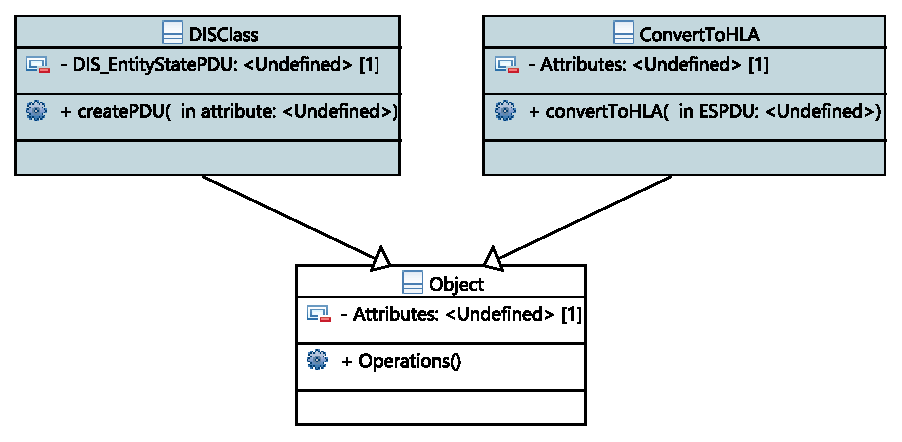
\includegraphics[scale=0.9]{bilder/pdfvorlagen/ansatz2}
	\caption[Ansatz 1]{Ansatz 1}
	\label{ansatz1}
\end{figure}
Der zweite Ansatz bestand darin, eine unabhängige Klassenhierarchie zu erstellen. Diese Hierarchie soll ihre eigenen Attribute und Methoden besitzen. Wie auch im ersten Ansatz, besitzt der zweite Ansatz eine Klasse \glqq Object\grqq{}. Zusätzlich existieren hier weitere Klassen, deren Elternklasse die Klasse \glqq Object\grqq{} ist. Diese besitzt jetzt als Attribut eine \ac{espdu} und zusätzlich noch Attribute, die allgemein für ein Objekt benötigt werden. Die spezifischen Attribute sind  in den  Kindklassen enthalten. \\  Wie in Bild \ref{ansatz2} zu sehen, wird zunächst unterschieden, ob ein Objekt beweglich oder starr an einem Ort ist. Ist ein Objekt mobil, wird unterschieden, ob es sich um ein ziviles oder militärisches Objekt handelt. Die Klassen \glqq civil\grqq{} und \glqq military\grqq{} stellen die unterste Ebene dar und erben, wie im Bild \ref{ansatz2} gezeigt, die Inhalte der Elternklassen. Die Entscheidung, ob ein Objekt beweglich oder starr an einem Ort ist, muss vorgenommen werden, da mobile Objekte sich fortbewegen können und demnach mindestens ein Attribut und die dazugehörigen Interface- und Verarbeitungsmethoden mehr hat als ein festes Objekt. Eine dieser  Verarbeitungsmethoden wäre die Berechnung der Positionsänderung in Abhängigkeit der Richtung, Geschwindigkeit und der Zeit. Die Entscheidung, ob ein Objekt zivil oder militärisch ist, wird benötigt, da sie sich grundlegend unterscheiden. Ein militärisches Objekt kann zum Beispiel aktiv an Kampfhandlungen teilnehmen, wohingegen ein ziviles Objekt maximal passiv daran teilnehmen kann. Durch die  Möglichkeit, aktiv an Kampfhandlungen teilzunehmen, kann das militärische Objekt Waffen besitzen, welche ihm die Teilnahme ermöglichen. Dies hat zur Folge, dass die dafür benötigten Attribute und Interface-Methoden in der Klasse implementiert werden. Des Weiteren werden Methoden benötigt, die das Schießen berechnen und simulieren. \\
Bei diesem Ansatz wird durch Methoden eine \ac{dis} \acl{espdu} erstellt, welche als Attribut in der Klasse \glqq Object\grqq{} gespeichert werden. Diese kann dann an andere Teilnehmer der Simulation gesendet werden. Parallel kann dazu auch eine Methode implementiert werden, die die gespeicherten Daten in \ac{hla} oder in eine andere Simulationsumgebung  konvertiert. \ac{dis} und \ac{hla} dienen hier nur als Schnittstelle zu anderen Simulationen. 
\begin{figure}[H]
	\centering
	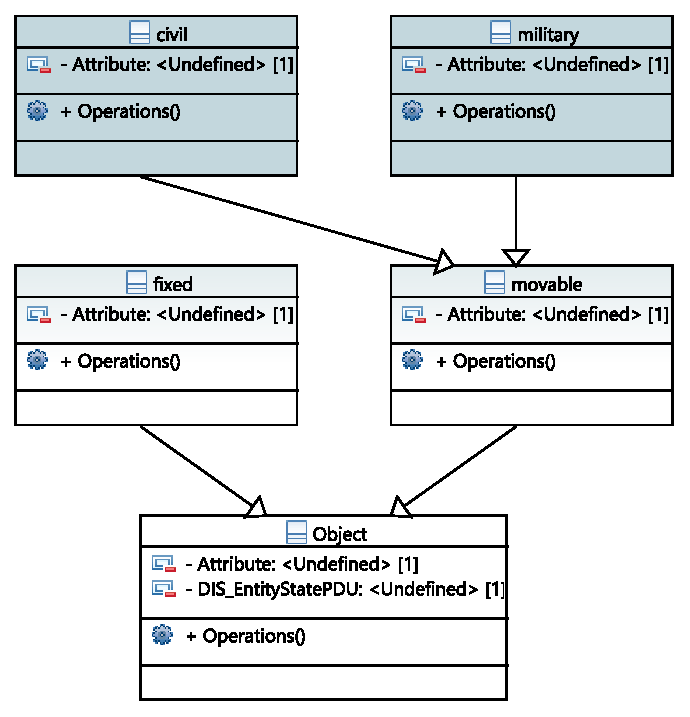
\includegraphics[scale=0.9]{bilder/pdfvorlagen/ansatz1}
	\caption[Ansatz 2]{Ansatz 2}
	\label{ansatz2}
\end{figure}
Der dritte Ansatz greift das Konzept des Zweiten auf, verfolgt jedoch eine andere Strategie. Im Bild \ref{ansatz3}, welches aufgrund der Größe im Anhang zu finden ist, wird das zum Ansatz gehörige \ac{uml} Diagramm gezeigt. Auch hier ist die Elternklasse, von der geerbt wird, die Klasse \glqq Object\grqq{}. In diesem Ansatz, wird eine grundlegend andere Unterscheidung vor genommen. Hier wird zunächst zwischen Objekten unterschieden, die sich selbständig und nicht selbständig fortbewegen können. Objekte, die sich von selbst bewegen können,  besitzen eine Geschwindigkeit und eine Richtung, in die das Objekt zeigt. Objekte, die sich nicht selbst bewegen können, können jedoch auch eine Geschwindigkeit besitzen beziehungsweise sie können sich auch fortbewegen. Der Unterschied dabei ist jedoch, dass es sich bei diesen Bewegungen entweder um einmalige Positionsänderung handelt oder um sehr kleine und daher vernachlässigbare Bewegungen. Ein Beispiel für ein Objekt, dass ein Objekt der Klasse \glqq nonDriven\grqq{} ist, sind Bojen. Bojen bewegen sich im Idealfall nicht oder nur sehr wenig. Die Positionsänderung wird daher nur über das Setzen einer neuen Position und nicht über eine Berechnung aus Geschwindigkeit, Zeit und Richtung vorgenommen. Von der Klasse  \glqq nonDriven\grqq{} sind die Klassen \glqq movable\grqq{} und   \glqq fixed\grqq{} abgeleitet. Der Unterschied zwischen den beiden Klassen besteht darin, dass sich bei der Klasse  \glqq movable\grqq{} die Position ändern kann und es deshalb Methoden existieren müssen, die die Position anpassen können. Bei der Klasse \glqq fixed\grqq{} wird vorausgesetzt, dass sich die Position nie ändern.\\
Die Klasse \glqq driven\grqq{} ist eine Kindklasse von der Klasse  \glqq Object\grqq{} und stellt das Gegenstück zur Klasse \glqq nonDriven\grqq{} dar. Sie ist die Elternklasse aller Klassen, die Objekte darstellen, die sich selbstständig fortbewegen können. Anschließend  wird zwischen Luftfahrzeugen, Landfahrzeugen, Seefahrzeugen und Unterseefahrzeugen unterschieden. Für jede Domäne existiert eine eigene Klasse. Diese Unterscheidung ist sinnvoll, denn dadurch können für jede Domäne spezifische Methoden erstellt werden, die zum Beispiel die Positionsangaben prüfen und dann gegebenenfalls Konsequenzen daraus ziehen. Des Weiteren kann dadurch das Objekt der Klasse genauer simuliert werden, es können beispielsweise Methoden implementiert werden, die die Flugbahn eines Flugzeugs oder die einer Rakete berechnen. Diese Methode darf jedoch nicht auf ein Objekt der Klasse \glqq Surface\grqq{}, \glqq Subsurface\grqq{} und \glqq Land\grqq{} angewendet werden. Die  Unterscheidung  zwischen militärischen und zivilen Objekten wird in jeder der Kindklassen  der Klasse \glqq driven\grqq{} getroffen. Dies hat zur Folge, dass jeweils zwei weitere Klassen hinzukommen, die jeweils das zivile und das militärische Objekt darstellen. Wie im Ansatz 2 beschrieben, ist das sinnvoll, da militärische Objekte andere Methoden und Attribute besitzen als ein ziviles Objekt.
Bei diesem Ansatz wird wie im Ansatz 2 die \ac{espdu} als Attribut in der Klasse \glqq Object\grqq{} gespeichert und dann gegebenenfalls an andere Teilnehmer verteilt.\\
Ein weiterer wichtiger Teil dieser Ansätze ist das Hinzufügen von Ausrüstung, da diese ein Objekt erst einsatzfähig macht. Dafür wurde eine Klassenhierarchie entwickelt, die der Grundidee der Ansätze 2 und 3 entspricht. Diese Klassenhierarchie ist im Anhang im Bild \ref{ausrüstung} zu finden. Die Klasse \glqq Equipment\grqq{} spiegelt die Ausrüstung wieder, die ein Objekt besitzt. Sie kann als Attribut in einer der beliebigen Klassen eingefügt werden.  Diese Klasse besitzt als Attribute zwei Container, in diesem Beispiel zwei Arrays, in denen jeweils alle vorhandenen Waffen und Sensoren gespeichert werden und einen String, in dem der Name gespeichert wird.  Dazu besitzt sie Methoden, mithilfe derer auf die Waffen und Sensoren zugegriffen werden kann. Dabei werden Methoden der Polymorphie benutzt, welche im Abschnitt  \ref{poly} beschrieben wurden. Des Weiteren wurde eine Klasse \glqq Weapon\grqq{} erstellt, welche die Elternklasse für die spezifischen Waffenklassen darstellt. Außerdem wurde eine Klasse \glqq Munition\grqq{} erstellt, welche als Elternklasse für die Munitionsklassen darstellt. Die derzeitig verfügbaren Waffenklassen sind die Klassen \glqq Cannon\grqq{} und \glqq Vls\grqq{}. Die Klasse \glqq Cannon\grqq{} stellt eine Rohrwaffe dar, die als Attribut einen Array der Klasse  \glqq Bullet\grqq{} besitzt. Die Klasse \glqq Vls\grqq{} stellt ein  \ac{vls} , eine Senkrechtstartanlage für Flugkörper, dar. Dieses System besitzt als Munition Raketen, welche mithilfe der Klasse \glqq Rocket\grqq{} dargestellt werden.  Die Raketen werden, wie in der Klasse \glqq Cannon\grqq{}, in einem Container gespeichert und verwaltet. Da sich die Munition der Waffenklassen grundsätzlich ähneln, sind die Klassen \glqq Bullet\grqq{} und  \glqq Rocket\grqq{}  von der Klasse  \glqq Munition\grqq{} abgeleitet. Neben den Waffenklassen existieren auch Sensorenklassen. Dazu gehören die Klassen \glqq Camera\grqq{}, \glqq Sonar\grqq{} und \glqq Radar\grqq{}. Diese Klassen werden wie Waffenklassen behandelt. 
 
\section{Vergleich der verschiedenen Lösungsansätze} 
Im folgenden Abschnitt werden die im vorhergehenden Abschnitt erklärten Ansätze miteinander verglichen. Es wird eine Bewertung der einzelnen Ansätze vorgenommen und abschließend wird der verwendete Ansatz genannt und es werden die Gründe für die Wahl dargestellt.\\
Der erste Ansatz ist, wie oben beschrieben, dem \ac{dis} sehr nahe. Vorteile dieses Ansatzes wäre, dass die Umsetzung sehr schnell wäre, und dass man sich nahe am \ac{dis} Standard bewegt, was die Teilnahme an \ac{dis} basierten Simulationen einfach gestalten würde. Nachteil dieses Ansatzes ist, dass man von dem jeweiligen Standard abhängig ist. Des Weiteren kann man bei diesem Ansatz nur anhand des Inhalts der \ac{espdu} unterscheiden, um was für ein Objekt es sich handelt. Dies hat zur Folge, dass nicht gewährleistet werden kann, dass  spezifische Objekte wie Schiffe, Flugzeuge oder Landfahrzeuge nur auf die für sie geltenden Methoden zugreifen können und somit die Methoden selbst prüfen müssen, um was für ein Objekt es sich handelt und dann entsprechende Berechnungen durchführt. Die Methoden, die für die speziellen Einsatzräume gelten, sind zum Beispiel Flugbahnberechnungen, Berechnungen, die die Position überprüfen oder Methoden zur Routen Berechnung.    \\
Der zweite  Ansatz hat den Vorteil, dass er von jedem Simulationsstandard losgelöst ist. Er enthält zwar als Attribut eine \ac{espdu}, jedoch kann diese nur bei Bedarf erstellt werden. Die Attribute, die in den Klassen enthalten sind, sind vom \ac{dis} Standard losgelöst. Bei der Erstellung  einer  \ac{espdu} werden diese Attribute übersetzt und in der entsprechenden Form in der \ac{espdu} gespeichert. Diese \ac{pdu} wird ausschließlich zur Kommunikation mit anderen Teilnehmern verwendet. Ein Nachteil dieses Ansatzes ist, dass nicht unterschieden wird, um was es sich bei diesem Objekt handelt. Es wird zwar unterschieden, ob es sich um ein ziviles oder militärischen Objekt handelt, jedoch werden beispielsweise militärische Schiffe, Flugzeuge und Landfahrzeuge gleich behandelt. Sie können, wie im Ansatz 1, auf die gleichen Methoden zugreifen, welche auch hier anhand von Attributen entscheiden müssen, um was für ein Objekt es sich handelt. \\
Im dritten Ansatz wird konsequent zwischen zivilen und militärischen, Luft-, Land- und Seeeinheiten unterschieden. Hier können zwar die militärischen und zivilen Einheiten auf die gleiche Elternklasse zugreifen, die Methoden für den jeweiligen Einsatzraum enthält. Jedoch können sie nicht auf Methoden zugreifen, die zu einem Einsatzraum gehören. Da Objekte nur noch auf die für sie gedachten Methoden zugreifen können, müssen diese Methoden nicht mehr prüfen, ob sie auf dieses Objekt angewendet werden dürfen. Die Implementierung dieser Methoden ist somit weniger komplex. Nachteile dieses Ansatzes sind, dass es für jedes Objekt des Einsatzraums jeweils eine Klasse für zivile und militärische Objekte gibt, was die Anzahl der Attribute und Methoden vergrößert. Des Weiteren  muss bei diesem Ansatz mehr darauf geachtet werden, dass Attribute und Methoden  nicht doppelt implementiert sind, da dies den Quellcode unnötig unübersichtlich und komplex machen würde. 
\\
Vergleicht man die Ansätze miteinander, fällt auf, dass die Anzahl der Klassen mit jedem Ansatz gestiegen ist. Des Weiteren muss man bei der Erstellung eines Objektes genau wissen, um was es sich handeln soll.
Beim ersten Ansatz kann man eine \ac{espdu} mit den entsprechenden Werten erstellen, ohne zu entscheiden, um was es sich bei dem Objekt handeln soll. Bei zweiten Ansatz muss man zwischen festen und beweglichen Objekten und wenn es sich um ein bewegliches Objekt handeln soll, ob es ein militärischen oder ziviles Objekt handelt, entscheiden. Beim dritten Ansatz kann man sich nur für ein Objekt entscheiden, welches auch als Klasse abgebildet ist. Benötigt man ein Objekt einer nicht vorhandenen Klasse, muss man den Ansatz um die benötigte Klasse erweitern. Diese Einschränkung bei der Auswahl ermöglicht es, immer die korrekten Methoden auf die Objekte anzuwenden. Der erhöhte Implementierungsaufwand ermöglicht jedoch eine sichere und korrekte Benutzung. 
Abschließend stellt sich der dritte Ansatz als der beste heraus, da bei der Implementierung der Methoden nicht auf einen unzulässigen Gebrauch geprüft werden muss, da die Methode immer nur von dem Objekt benutzt werden kann, für das sie bestimmt ist. Für die Implementierung wurde daher dieser Ansatz genutzt, da die Implementierung der Methoden die einfachere ist und weil sich dieser Ansatz auf Grund seiner Struktur  potentiell am  besten erweitern lässt.  

\section{Implementierung}\label{implement}
Die Klassenhierarchie wurde mithilfe eines \ac{uml} Diagramms entworfen, welches mit der Papyrus Erweiterung der Eclipse \ac{ide} erstellt wurde. Anhand dieses Diagramms wurde eine C++ Projekt generiert, das anschließend vervollständigt wurde. Dabei wurden weitere Methoden und Attribute hinzugefügt. Bei der Implementierung traten einige Probleme auf. Die Komplexesten werden im folgenden Abschnitt aufgezeigt und es wird die implementierte Lösung erklärt.\\
Die erste Aufgabe war es alle \glqq get\grqq{} und \glqq set\grqq{} Methoden zu implementieren.  
Im Listing \ref{getset} ist eine einfache Implementierung dieser Methoden zu sehen. Hier wird das Attribut \glqq Type\grqq{}, welches \glqq private\grqq{} ist, gesetzt und abgerufen. Die unten gezeigte Implementierung ist beispielhaft für die anderen Methoden. 
\begin{lstlisting}[caption =\glqq get\grqq{} und \glqq set\grqq{} Methode ,label=getset]
void driven::setType(std::string /*in*/type) {
Type = type;
}
std::string driven::getType() {
return Type;
}
\end{lstlisting}

Das nächste Problem war es die Konstruktoren zu erstellen. Hierbei galt es zunächst diese so einfach wie möglich zu halten. Jedoch wurde schnell sichtbar, dass die Eingaben überprüft werden müssen. Der Grund dafür entstand aus der Forderung, dass ein Objekt in den \ac{dis} Standard übersetzt werden soll. Da \ac{dis} über eine Enumeration verfügt, in der die verschiedenen Arten einer Entity kodiert sind, muss das Programm erkennen, wie es das vorhandene Objekt übersetzen kann, sodass es zu einem der Objekte passt, die in der Enumeration kodiert sind. Um dies zu erfüllen, wurde entschieden, dass es am besten wäre, diese Prüfung direkt im Konstruktor vorzunehmen und diese als String zu speichern, um die Lesbarkeit beizubehalten.   
\begin{lstlisting}[caption =Konstruktor  \glqq warShip\grqq{} Klasse ,label=warshipclass]
warShip::warShip(std::string /*in*/Name,
std::string /*in*/Type, std::string/*in*/ Country) {
object::setName(Name);
object::setCountry(Country);
object::setKind("Platform");
object::SetDomain("Surface");
object::setPosition(0,0,0);
object::incrementCounter();
driven::setType(Type);
equipment = NULL;
if (Type== "F124") {
  driven::setCategory("Guided Missile Frigate (FFG)");
  driven::setSubCategory("Sachsen Class (Type 124)");
} else if (Type == "F123") {
  driven::setSubCategory("Brandenburg class (Type 123)");
  driven::setCategory("Guided Missile Frigate (FFG)");
}else if (Type == "F122"){
  driven::setSubCategory("Bremen class (Type 122)");
  driven::setCategory("Guided Missile Frigate (FFG)");
} else{
  std::string SubCategory , Category;
  std::cout <<"Category as written in DIS Enum:";
  getline(std::cin, Category);
  std::cout <<"SubCategory as written in DIS Enum:"
  << std::endl;
  getline(std::cin, SubCategory);
  driven::setSubCategory(SubCategory);
  driven::setCategory(Category);
}}
\end{lstlisting}
Im Listing \ref{warshipclass} ist der Konstruktor der Klasse \glqq warShip\grqq{} dargestellt. Hier ist zu sehen, dass für das Erstellen der Klasse nur die Attribute \glqq Name\grqq{}, \glqq Type\grqq{} und \glqq Country\grqq{} dem Konstruktor übergeben werden. Neben den genannten Attributen werden noch weitere benötigt, die das Objekt noch genauer spezifizieren.
Die weiteren Attribute sind  \glqq Category\grqq{}, \glqq SubCategory\grqq{}, \glqq Kind\grqq{} und  \glqq Domain\grqq{}. Diese weiteren Attribute sind jedoch nur für die korrekte Erstellung der \ac{espdu} notwendig.
Die Attribute   \glqq Category\grqq{} und \glqq SubCategory\grqq{} sind \ac{dis} spezifisch und sollten möglichst dem Inhalt der Enumeration entsprechen, da sonst die Übersetzung nicht möglich ist. 
Die hier gezeigt Implementierung ist jedoch nur zu Testzwecken. Eine andere Lösung wäre die Erstellung einer Datenbank beziehungsweise eines Containers, in dem die möglichen Werte für die Attribute gespeichert sind und das Anhand des  \glqq Type\grqq{}  Wertes entschieden wird, welche Werte die Attribute  \glqq Category\grqq{} und \glqq SubCategory\grqq{} erhalten. Die Konstruktoren der Klassen  \glqq warPlane\grqq{},\glqq civilPlane\grqq{}, \glqq military\grqq{}, \glqq civil\grqq{} und \glqq civilShip\grqq{} können auf die gleiche Weise implementiert werden, wobei das für die Klassen \glqq military\grqq{} und \glqq warPlane\grqq{} schon der Fall ist.\\
Das wohl komplexeste Problem war die Übersetzung eines Objektes in eine \ac{espdu}. Dafür wurde eine eigene Klasse erstellt, die nur dafür zuständig ist, den \glqq Entity Type\grqq{} zu erstellen. Diese Klasse enthält eine Datenbank, die aus der \ac{dis} Enumeration entnommen wurde. 

\begin{lstlisting}[caption = Ausschnitt DIS\_enum.h  ,label= disenum]
class DIS_enum {
public:
DIS_enum();
// ~DIS_enum();

DIS_EntityType_Variables getDISEntityType(std::string kind,
   std::string domain, std::string country,
   std::string category,  std::string subcategory, 
   std::string specific,  std::string extra);

private:
std::map<int,std::string> Kind;
std::map<int,std::string> DomainPlatform;
std::map<int,std::string> DomainMunition;
std::map<int,std::string> Country;
std::map<int,std::string> CategoryLand;
std::map<int,std::string> CategoryAir;
std::map<int,std::string> CategorySurface;

...
};
\end{lstlisting}
Das Listing \ref{disenum} ist ein Ausschnitt der Header Datei der \glqq DIS\_enum \grqq{} Klasse. In Zeile 6 ist die Funktion zusehen, die mithilfe der eingegebenen Strings einen Struct befüllt, mit dessen Hilfe das   \glqq Entity Type \grqq{} Feld befüllt wird. Bevor jedoch diese Funktion genutzt werden kann, muss zunächst der Konstruktor aufgerufen werden. Dieser dient zur Erstellung eines Objektes und zur Befüllung der Container, in diesem Fall der vorhandenen Maps. In Listing \ref{disenumcpp} ist ein Teil des Konstruktors abgebildet. Dieser Teil zeigt wie die Maps befüllt werden.
 \begin{lstlisting}[caption = Ausschnitt DIS\_enum.cpp  ,label= disenumcpp]
DIS_enum::DIS_enum(){
Kind[0]="Other";
Kind[1]="Platform";
Kind[2]="Munition";
Kind[3]="Life form";
 
 
DomainPlatform[0]="Other";
DomainPlatform[1]="Land";
DomainPlatform[2]="Air";
DomainPlatform[3]="Surface";
DomainPlatform[4]="Subsurface";
...
}
 \end{lstlisting}
 Die Maps, die derzeit erstellt wurden, können in der Header Datei gefunden werden. Diese Maps sind nur teilweise vollständig befüllt. Falls ein benötigter Eintrag nicht vorhanden ist, können die benötigten Werte in der \ac{dis} Enumeration \cite{Shanks.} gefunden werden. \\ \newpage
 Die in Listing \ref{disenum} zu sehende Funktion \glqq DIS\_EntityType\_Variables getDISEntityType()\grqq{} 
hat als Rückgabewert einen Struct, der Folgenden Integer Werte beinhaltet: 
\begin{itemize}
	\singlespacing
	\item Kind
	\item Domain
	\item Country
	\item Category
	\item SubCategory
	\item Specific
	\item Extra
\end{itemize}
Der Inhalt entspricht dem  des \glqq Entity Type\grqq{} Feldes. Als Input Parameter werden der Funktion die in Listing  \ref{disenum} zu sehenden Strings übergeben. Da die Werte des \glqq Entity Type\grqq{}  von einander abhängen, ist die Struktur der Funktion die eines Baumes.  In Listing \ref{funcpart1} ist die erste Entscheidung zusehen. Es wird zunächst geprüft, um was es sich bei dem Objekt grundlegend handelt. Es wird zwischen \glqq Platform\grqq{}, \glqq Munition\grqq{}, \glqq Life form\grqq{},\glqq Environmental\grqq{} und Anderen entschieden. Genauere Informationen sind in der Enumeration enthalten \cite{Shanks.}. Diese Information ist im Attribut \glqq Kind \grqq{} gespeichert. In der derzeitigen Version der Funktion ist nur der \glqq case 1\grqq{} implementiert. 
 \begin{lstlisting}[caption = Funktion \glqq getDISEntityType()\grqq{} Teil 1  ,label= funcpart1]
for (std::map<int,std::string>::iterator it=Kind.begin(); 
     it!=Kind.end(); ++it)
if (it->second == kind) {
help.Kind =  it->first;
}
switch (help.Kind) {
case 1: // platform
  for (std::map<int,std::string>::iterator 
       it=DomainPlatform.begin(); it!=DomainPlatform.end();
       ++it)
  if (it->second == domain) {
  help.Domain =  it->first;
  }
  switch (help.Domain) { ... }
break;
case 2: // munition
break;
...
default : std::cout << "invalid Kind" << '\n';
std::cout << "Possible is: 'Other'  'Platform'  'Munition'
'Life form'  'Environmental'  'Cultural Feature'  'Supply'
'Radio'  'Expendable' or 'Sensor/Emitter' " << '\n';
}
\end{lstlisting}
 Trifft der Fall nun zu, so wird nun die Domäne geprüft, also ob es sich um ein Land, Luft, See oder Untersee Objekt handelt. Diese Information ist im String \glqq Domain \grqq{} gespeichert. In der vorliegenden Version sind nur die Fälle implementiert, in denen die Domäne Land oder Surface ist. Die anderen Fälle müssen noch implementiert werden. Trift einer der Fälle zu, wird nun geprüft, welchem Land das Objekt angehört. 
 \begin{lstlisting}[caption = Funktion \glqq getDISEntityType()\grqq{} Teil 2  ,label= funcpart2]
switch (help.Domain) {
case 0: // domain other
break;
case 1: // land
  for (std::map<int,std::string>::iterator 
       it=Country.begin(); it!=Country.end(); ++it){
  if (it->second == country) {
  help.Country =  it->first;
  }  }
  switch (help.Country) {...}
break;
case 2: // air
break;
case 3: // surface
...
break;
...
default: ...
 \end{lstlisting}
 Hier kann zwischen den USA, Russland und Deutschland entschieden werden. Sollen weitere Nationen verfügbar sein, muss die entsprechende Map angepasst werden. 
\begin{lstlisting}[caption = Funktion \glqq getDISEntityType()\grqq{} Teil 3  ,label= funcpart3]
switch (help.Country) {
case 78: // germany
for (std::map<int,std::string>::iterator 
     it=CategoryLand.begin(); it!=CategoryLand.end(); ++it){
if (it->second == category) {
help.Category =  it->first;
} }
switch (help.Category) {
  case 1 : // tank
     for (std::map<int,std::string>::iterator 
          it=GermanLandTankSubcategory.begin(); 
          it!=GermanLandTankSubcategory.end(); ++it){
     if (it->second == subcategory) {
     help.SubCategory =  it->first;
     }   }
  break;
  case 2 : // amored fighting vehicle
  break;
  case 3 : // armored Utility Vehicle
  break;
  default: std::cout << "invalid Category" << '\n';
  break;
  }
break;
case 225: 
...
break;
...
\end{lstlisting}
 In Listing \ref{funcpart3}  ist dargestellt, wie in der Domäne  \glqq land\grqq{}, der Nation  \glqq germany\grqq{} und in der Kategorie  \glqq tank\grqq{} die Unterkategorie übersetzt wird. Die Implementierung für die anderen verfügbaren Nationen sind analog zu der gezeigten Implementierung.
 An diesem Punkt wurden die Werte für  \glqq Kind\grqq{},\glqq Domain\grqq{},\glqq Country\grqq{}, \glqq Categrory\grqq{} und \glqq SubCategrory\grqq{} übersetzt.  Die Werte für \glqq Specific\grqq{} und \glqq Extra\grqq{} werden nicht gesetzt, da  diese die genauen Versionen der Modelle wieder spiegeln und das in dem Rahmen der Masterarbeit nicht nötig war. Eine Erweiterung um diese beiden Werte wäre ohne großen Aufwand möglich. \\ Die beschriebene Funktion ist jedoch nur ein Teil bei der Erstellung einer  \ac{espdu}.  
 Eine weitere Funktion ist die \glqq makeDISArticulationsParameter()\grqq{}. Diese Funktion übersetzt die Ausrüstung in das \ac{dis} Format. \\ 
 Die Waffen und Sensoren werden in der \glqq Equipment\grqq{} Klasse und zwei unterschiedlichen Listen speichert. Das Überführen in das \ac{dis} Format erfolgt deshalb getrennt voneinander.
 \begin{lstlisting}[caption = ArticulationParameter  ,label= param1]
std::list<Model::weapon*> weapon = equipment->getWeapon();
std::list<Model::sensor*> sensor = equipment->getSensor();
int amountTurrents = 0;
int amountLauncher = 0;
int amountRadars = 0;
int amountSonar = 0;

for(std::list<Model::weapon*>::iterator it=weapon.begin();
    it != weapon.end(); it++)
{
if((*it)->getType()=="PRIMARY_TURRET"){
  DIS::ArticulationParameter DISequipment[3];
  ...
  amountTurrents++;
} else if ((*it)->getType()=="VLS") {
  DIS::ArticulationParameter DISequipment;
  ...
  amountLauncher++;
} else{
  // more weapons
}
}
for(std::list<Model::sensor*>::iterator it=sensor.begin(); 
    it != sensor.end(); it++)
{
 if((*it)->getType()=="RADAR"){
  DIS::ArticulationParameter DISequipment[1];
 ...
 amountRadars++;
} else if ((*it)->getType()=="SONAR") {
 DIS::ArticulationParameter DISequipment;
 ...
 amountSonar++;
}else {
// more sensors
}}
 \end{lstlisting}
In Listing \ref{param1} ist das Gerüst der Funktion gesehen. Als ersten werden sämtliche Waffen und Sensoren eines Objektes abgefragt und zwischen gespeichert. Anschließend werden die Listen nach den entsprechenden Arten der Waffen durchsucht, wobei für jede Art gesondert verfahren wird. Dies wird mit einer \glqq if()\{\} else if()\{\}\grqq{} Kaskade realisiert. Ein \glqq switch case \grqq{} ist nicht möglich, da hier Strings verglichen werden. Die Zählvariablen werden benötigt, da jede Waffe und jeder Sensor eine spezielle Kennung in Abhängigkeit der Anzahl besitzt. In der hier gezeigten Version sind nur zwei verschiedene Waffen und zwei verschiedene Sensoren implementiert. Weitere können einfach durch Erweiterung der  \glqq if()\{\} else if()\{\}\grqq{} Kaskade eingefügt werden. Außerdem müssen die Enumerationen, die in Listing \ref{enum} gezeigt sind, erweitert werden. 
\begin{lstlisting}[caption = Parameter Enumeration ,label= enum]
namespace Articulation
{
enum Motion
{
  AZIMUTH = 11,
  AZIMUTH_RATE = 12,
  ELEVATION = 13,
  POSITION = 1
};
enum Part
{
  PRIMARY_TURRET = 4096,
  PRIMARY_GUN = 4416,
  SECONDARY_GUN = 6016,
  PRIMARY_LAUNCHER = 4736,
  PRIMARY_RADAR = 5376,
  SECONDARY_RADAR = 6976
};
enum Designator
{
  ARTICULATED = 0,
  ATTACHED = 1
};}
\end{lstlisting}

Die Anzahl der Parameter, die für eine bestimmte Waffe oder Sensor genutzt werden, hängt zum Einen von der Waffe oder dem Sensor ab, die übersetzt werden und zum Anderen von der geforderten Detailgenauigkeit. Hier gilt der Grundsatz, je detaillierter desto mehr Parameter werden benötigt. In der gezeigten Funktionen werden für eine Kanone drei Parameter und für das \ac{vls} ein Parameter  erstellt. Die Sensoren werden je durch einen Parameter dargestellt.\\ 
Neben den beschriebenen Funktionen zur Erstellung des \glqq Entitiy Type\grqq{} und zur Übersetzung des Equipments wurde noch zwei weitere Funktionen erstellt. Eine der Funktionen, die  \glqq makeStdDISPDU(DIS::Vector3Float velo,DIS::Orientation orie)\grqq{}, ist für das Hinzufügen der globalen Variablen, wie der Protokoll Version, der ExerciseID, der EntityID und der ForceID. Des Weiteren fügt sie alle Informationen zur \ac{espdu} hinzu, die von anderen Funktionen erstellt wurden. Dazu gehören der \glqq Entitiy Type\grqq{}, die Position, die Geschwindigkeit und die Orientierung, wobei sie die Geschwindigkeit und die  Orientierung als Input erhält und nur zur \ac{espdu} hinzufügt. Die beiden Informationen sind Bestandteil der Klasse \glqq driven\grqq{} und müssen daher übergeben werden. Die EntityID und die ForceID stellen eine Besonderheit dar. Da mithilfe dieser Klassenhierarchie mehrere Objekte erstellt werden soll, die an einer Simulation teilnehmen, muss die Vergabe der EntityID und der ForceID dynamisch erfolgen.  
Dazu wurden vier statische Zählvariablen und eine boolsche Variable erstellt. Die Zählvariablen zählen die erstellten Objekte und die Anzahl der Objekte, die Freund, Feind oder Neutral sind. Die boolsche Variable wird nach der erstmaligen Erstellung der ForceID und EntityID auf \glqq TRUE\grqq{} gesetzt, was das erneute Erstellen verhindert, denn eine ForceID und EntityID  muss für ein Objekt im laufe einer Simulation immer gleich bleiben. In \ac{dis} erhalten freundliche, feindliche und neutrale Objekte eine Unterschiedliche EntityID und ForceID. Diese ID's sind neben der Angehörigkeit auch von der laufenden Nummer des Simulationsobjektes abhängig. Für freundliche Entity's beginnt diese Zahl bei 1 und wird für jede weitere freundliche Entity um 3 erhöht. Bei feindlichen Entity's beginnt sie bei 2 und wird dann um 3 erhöht und bei neutralen beginnt sie bei 3 und wird anschließend für jede Weitere um 3 erhöht. Entity's, die weder freundlich noch feindlich noch neutral sind, erhalten als EntityID und ForceID eine 0. 
\begin{lstlisting}[caption = EntityID und ForceID ,label= id]
DIS::EntityID DISunit_entity_id;
DISunit_entity_id.setSite( 0 );
DISunit_entity_id.setApplication( 1 );
int ForceID;
if (Membership == "Other") {
  DISunit_entity_id.setEntity( 0 );
  ForceID = 0;
} else if(Membership == "Friendly") {
  DISunit_entity_id.setEntity( (1 + CounterFriendly * 3)-3 );
  ForceID = ((1 + CounterFriendly * 3)-3);
}else if(Membership == "Enemy"){
  DISunit_entity_id.setEntity( (2 + CounterEnemy * 3)-3 );
  ForceID = ((2 + CounterEnemy * 3)-3);
} else {
  DISunit_entity_id.setEntity( (3 + CounterNeutral * 3)-3);
  ForceID = ((3 + CounterNeutral * 3)-3);
}
...
if (EntityIDisSet == false) {
  DISUnit.setEntityID(DISunit_entity_id);
  DISUnit.setEntityType(DISType);
  DISUnit.setForceId(ForceID);
  EntityIDisSet = true;
}
\end{lstlisting}
In Listing \ref{id} ist die Implementierung der oben beschriebene Vergabe gezeigt.
\\
Die vierte und letzte Funktion ist die Funktion, mit der man das Erstellen und den Aufruf der anderen beschrieben Funktionen anstößt. Außerdem erstellt sie die \ac{dis} Vectoren, welche die Geschwindigkeit und die Orientierung beinhalten und übergibt diese an die Funktion \glqq makeStdDISPDU(DIS::Vector3Float velo,DIS::Orientation orie)\grqq{}. 
Die Funktionen, die zur Erstellung der \ac{espdu} benötigt werden, sind, mit Ausnahme der \glqq makeStdDISPDU(DIS::Vector3Float velo,DIS::Orientation orie)\grqq{} und der \glqq DIS\_EntityType
\_Variables getDISEntityType()\grqq{} Funktion, in der Klasse \glqq drvien \grqq{} implementiert. \\
Die \ac{espdu} kann mithilfe der Methode \glqq sendToNetwork(char DST[15]) \grqq{} an andere Teilnehmer gesendet werden. Als Input erhält die Methode die IP Adresse, an die gesendet werden soll. Die Daten werden mithilfe des \ac{udp} versendet.\\
Die letzte Mehtode, die erklärt wird, kann unter anderem das Fortbewegen der \ac{espdu} ermöglichen. 
Die Methode \glqq updateObject(double dt) \grqq{} erhält als Input eine Zeit in Sekunden, mit deren Hilfe die zurückgelegte Entfernung berechnet wird. 
 \begin{lstlisting}[caption = Update Funktion ,label= update]
position_dec position = object::getPosition();
Vector3D orientation = driven::getOrientation();
Vector3D velocity = driven::getVelo();
position_dec newPosition;

geod.Direct(position.lat,position.lon,
            orientation.x,velocity.x*dt,
            newPosition.lat,newPosition.lon);

object::setPosition(newPosition.lat,newPosition.lon,
		    position.height_above_geoid);
 \end{lstlisting}
 In  Listing \ref{update} ist die bisher implementierte Methode zusehen. Die verwendete Funktion, die in Zeile 6 zu sehen ist, stammt aus der GeographicLib. Diese Library wurde in der Studienarbeit \glqq Beurteilung der open-dis c++ Library zur simulation von militärischen szenarien\grqq{} \cite{HenryWinkel.} erklärt. Die aktuelle Version der  \glqq updateObject(double dt) \grqq{} Funktion, ermöglicht derzeit nur die geradlinige Fortbewegung. Die Methode soll später das gesamte Objekt updaten, sodass alle Parameter verändert werden können und dass diese immer den Korrekten Wert anzeigen.
 
 \section{Fähigkeiten der Klassenhierarchie}
Im folgenden Abschnitt wird beschrieben, was die fertige Klassenhierarchie für Möglichkeiten bietet. Die konkrete Implementierung wird für ausgewählte Methoden im Abschnitt \ref{implement} erklärt.
Grundlegend kann jedoch gesagt werden, dass die Klassenhierarchie eine Grundlage liefert, die je nach Bedarf beliebig erweitert werden kann.
Diese setzt sich aus dem Ansatz 3 und der Klassenhierarchie für die Ausrüstung zusammen. 
Mit der Klassenhierarchie ist es Möglich, ein Objekt zu erstellen, das ein ziviles oder militärischen Schiff, ziviles oder militärisches Flugzeug oder ein ziviles oder militärischen Landfahrzeug sein kann. Diesem Objekt können folgende Informationen gegeben werden:
\begin{itemize}
	\singlespacing
	\item Name
	\item Typ
	\item Kategorie
	\item Nation
	\item Fraktionsangehörigkeit
	\item Position
	\item Geschwindigkeit
	\item Lage
	\item Equipment
\end{itemize}
Neben den oben genannten Attributen besitzt ein Objekt noch weitere, die nicht vom User gesetzt werden müssen, da sich bei entsprechender Eingabe im Konstruktor automatisch gesetzt werden. Klassen, bei denen diese Attribute automatisch im Konstruktor gesetzt werden, sind die \glqq warShip\grqq{} und die \glqq military\grqq{} Klasse. Diese Möglichkeit wurde bei diesen Klassen experimentell implementiert.
Des Weiteren wurden eine Methode implementiert, mithilfe derer sich die Bewegung eines Objektes berechnen lässt. \\
Nach der Erstellung eines Objektes der Grundklassen, können auch Ausrüstungsobjekte erstellt werden, die dann anschließend einem Objekt der Grundklasse als Attribut hinzugefügt wird. Als Grundlage für die Ausrüstung wurde das Model genutzt, welches im Abschnitt \ref{lös} beschrieben ist. Hierbei wurde sich auf zwei Waffen und auf drei Sensoren beschränkt. Weitere Klassen können, wie bei den Beispielklassen gezeigt, hinzugefügt werden. \\
\begin{lstlisting}[caption = main.cpp ,label= main]
#include <iostream>

#include "warShip.h"
#include "cannon.h"
#include "rocket.h"
#include "vls.h"
#include "weapon.h"

#define DST "127.0.0.255"

int main(int argc, char const *argv[]) {
Model::warShip ship1("Hamburg","F124","Germany");
ship1.setMembership("Friendly");

Model::Equipment eq1("Alpha");
Model::cannon can1("Otto Melara MK21",120);
Model::vls vls1("VLS System",32 );
Model::rocket rocket("Tomahawk","Cruise missile",3000);

vls1.addRocket(&rocket);
eq1.addWeapon(&can1);
eq1.addWeapon(&vls1);
ship1.addEquipment(&eq1);

ship1.createDISPDU();
ship1.sendToNetwork(DST);
return 0;
}
\end{lstlisting}
In Listing \ref{main} ist die Main.cpp zusehen. Dieses Programm testet, soweit möglich, die Klassenhierarchie. Hier wird beispielsweise ein Kriegsschiff erstellt, mit Ausrüstung  bestückt und anschließend als \ac{espdu} an die angegebenen IP Adresse versendet.
In Zeile 12 ist die Erstellung eines Kriegsschiffes der F124 Klasse zusehen. Als weitere Parameter werden der Name sowie die Nation übergeben. In Zeile 13 wird die Gesinnung festgelegt.   In den Zeilen 15 bis 18 werden die Objekte für die Ausrüstung erstellt. In den Zeilen 20 bis 23 wird die erstellte Ausrüstung dem Schiff, beziehungsweise dem Objekt der Klasse \glqq Equipment\grqq{}, hinzugefügt. In Zeile 25 wird die Methode aufgerufen, die das erstellte Objekt in eine \ac{espdu} übersetzte. In der darauf folgenden Zeile wird die \ac{espdu} dann an die Adresse \glqq DST\grqq{} gesendet.\\ 
Das in Listing \ref{main} erstellte Objekt der Klasse \glqq warShip\grqq{} kann in der aktuellen Version der Klassenhierarchie durch ein Objekt der Klasse \glqq military\grqq{}, also durch ein militärisches Landfahrzeug ersetzt werden. Allgemein lässt sich sagen, dass nach der Implementierung der Konstruktoren und der Ergänzung der Datenbank der Klasse \glqq DIS\_enum\grqq{}, sich jedes beliebige Objekt erstellen, übersetzen und senden lassen kann.  

\section{Offene Probleme}\label{prob}
Wie in den vorhergehenden Abschnitten bereits angeschnitten, ist eines der offenen Probleme die Erweiterung der Datenbanken und Konstruktoren, die die Erstellung weiterer Objekte der verschiedenen Klassen ermöglichen. In der aktuellen Version wurden nur wenige Einheiten in der Datenbank aufgenommen, da lediglich das Grundgerüst geschaffen werden sollte und es keinen konkreten Bedarf gab. \\
Ein weiteres offenes Problem ist die Implementierung der Methoden, die die Position eines Objektes überprüfen und gegebenenfalls für ungültig erklären oder diese korrigieren.  Dies ist nötig, da verhindert werden muss, dass Schiffe eine Position haben, deren Koordinaten eine Höhe besitzt, welche nicht zu einem Schiff passt. Ein weiteres Beispiel ist das ein Landfahrzeug  keine Position haben darf, die auf eine Position auf dem Wasser oder unter dem Wasser hinweist. Dabei muss jedoch auf die Vorgabe der Simulation geachtet werden, da Landfahrzeuge prinzipiell unter Wasser sein können, jedoch diese Position ungewöhnlich für ein Landfahrzeug ist.\\
Ein anderes Problem ist das Implementieren einer Methode, die das Abfeuern einer Waffe simuliert. Das Abfeuern muss anschließend als \ac{pdu} an die Simulationsteilnehmer gesendet werden. Die Methode, die zum Beispiel das Feuern übersetzt, kann neu implementiert werden oder es kann die Methode der Klasse \glqq DIS\_enum\grqq{} erweitert werden. Neben dem Abfeuern einer Waffe wird dann auch die Simulation des Umsetzens beziehungsweise der Einschlag der Munition benötigt. Hierfür wird ebenfalls die entsprechende  \ac{pdu} benötigt.\\
Wie beschrieben, sollen mithilfe der Klassenhierarchie Objekte simuliert werden, die sich nicht eigenständig bewegen können. Hierfür müssen gegebenenfalls weitere Klassen hinzugefügt werden oder bestehende angepasst werden. Diese Möglichkeit wurde noch nicht implementiert, da Wert auf die Implementierung der Klassen gelegt wurde, die Kindklassen der Klasse  \glqq driven\grqq{} sind. \\
Ein weitere sinnvolle Erweiterung wäre beispielsweise die Implementierung von Methoden, die ein Objekt festgelegte Kurse abfahren oder fliegen lässt. Dabei muss überprüft werden, dass die eingegebenen Kurse zu den Objekten und deren Einsatzgebieten passen. 
\chapter{Fazit}
In dieser Masterarbeit wurden die Grundsätze der \acl{oop} und einige ausgewählte Besonderheiten der Programmiersprache C++ erklärt. Des Weiteren wurde der Inhalt einer \ac{espdu} erklärt. 
Außer den genannten Grundlagen, wurden die gefundenen Lösungsansätze erklärt und verglichen, die als Grundlage der Klassenhierarchie dienten. Im Anschluss dazu wurde die Implementierung wichtiger Methoden anhand des Quellcodes erklärt. Abschließend wurden die offenen Probleme genannt. \\
Die erstellte Klassenhierarchie bietet eine gute Grundlage für die Erstellung von Objekten. Um ein Objekt schlussendlich zu simulieren, fehlen jedoch noch einige wichtige Methoden. Für die Übersetzung eines Objektes in den \ac{dis} Standard  wurden Methoden erstellt mit denen man derzeit ausgewählte Objekte bestimmter Typen übersetzen kann. Eine Erweiterung dieser möglichen Typen ist relativ einfach zu realisieren. \\
Abschließend kann gesagt werden, dass die Klassenhierarchie die nötigen Grundlagen für Erweiterungen bietet. Sie ist von dem \ac{dis} Standard losgelöst, bietet jedoch Methoden, die es ermöglichen mit anderen Simulationen mithilfe des \ac{dis} Standards zu kommunizieren. Andere Standards können ebenfalls bereitgestellt werden. 


\chapter{Anhang}
%\begin{figure}[H]


\vspace{1cm}


%\begin{center}

%\begin{sidewaysfigure}[!h]
 
	%\begin{minipage}{\textwidth}
	\begin{figure}[h]

	\rotatebox{90}{%
		\centering
		\parbox{\textwidth}{%
%\begin{minipage}{0.75\textheight}
		\centering
	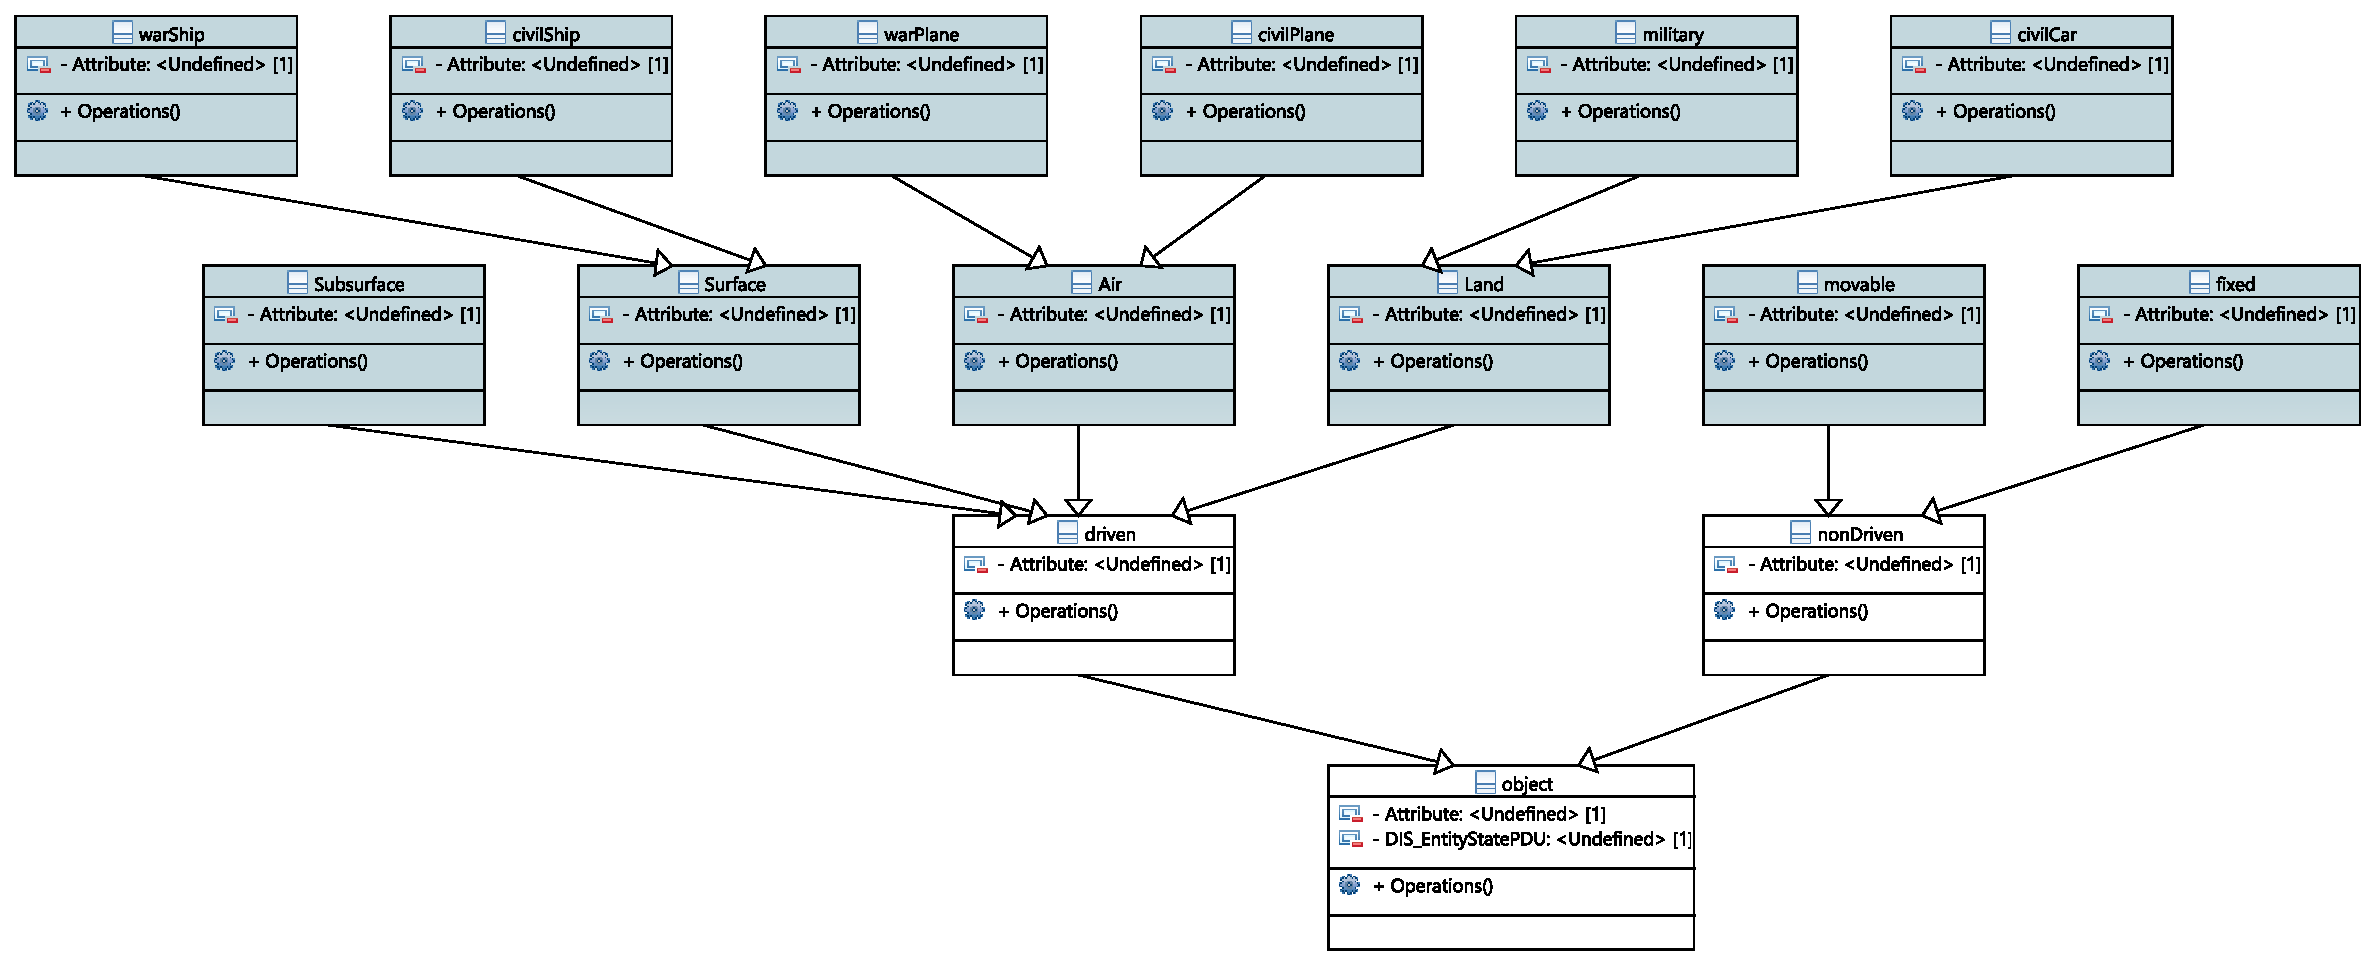
\includegraphics[height = 0.72 \textheight,width =1.1\textwidth]{bilder/pdfvorlagen/ansatz3}

	\caption[Ansatz 3]{Ansatz 3}
	

	\label{ansatz3}
  % \end{minipage}
%\end{minipage}
}
}
\end{figure}
%\end{center}


%\end{sidewaysfigure}

%\end{figure}

\begin{figure}[h]
	
	\rotatebox{90}{%
				\centering
		\parbox{1.5\textwidth}{%
			%\begin{minipage}{0.75\textheight}
			\centering
			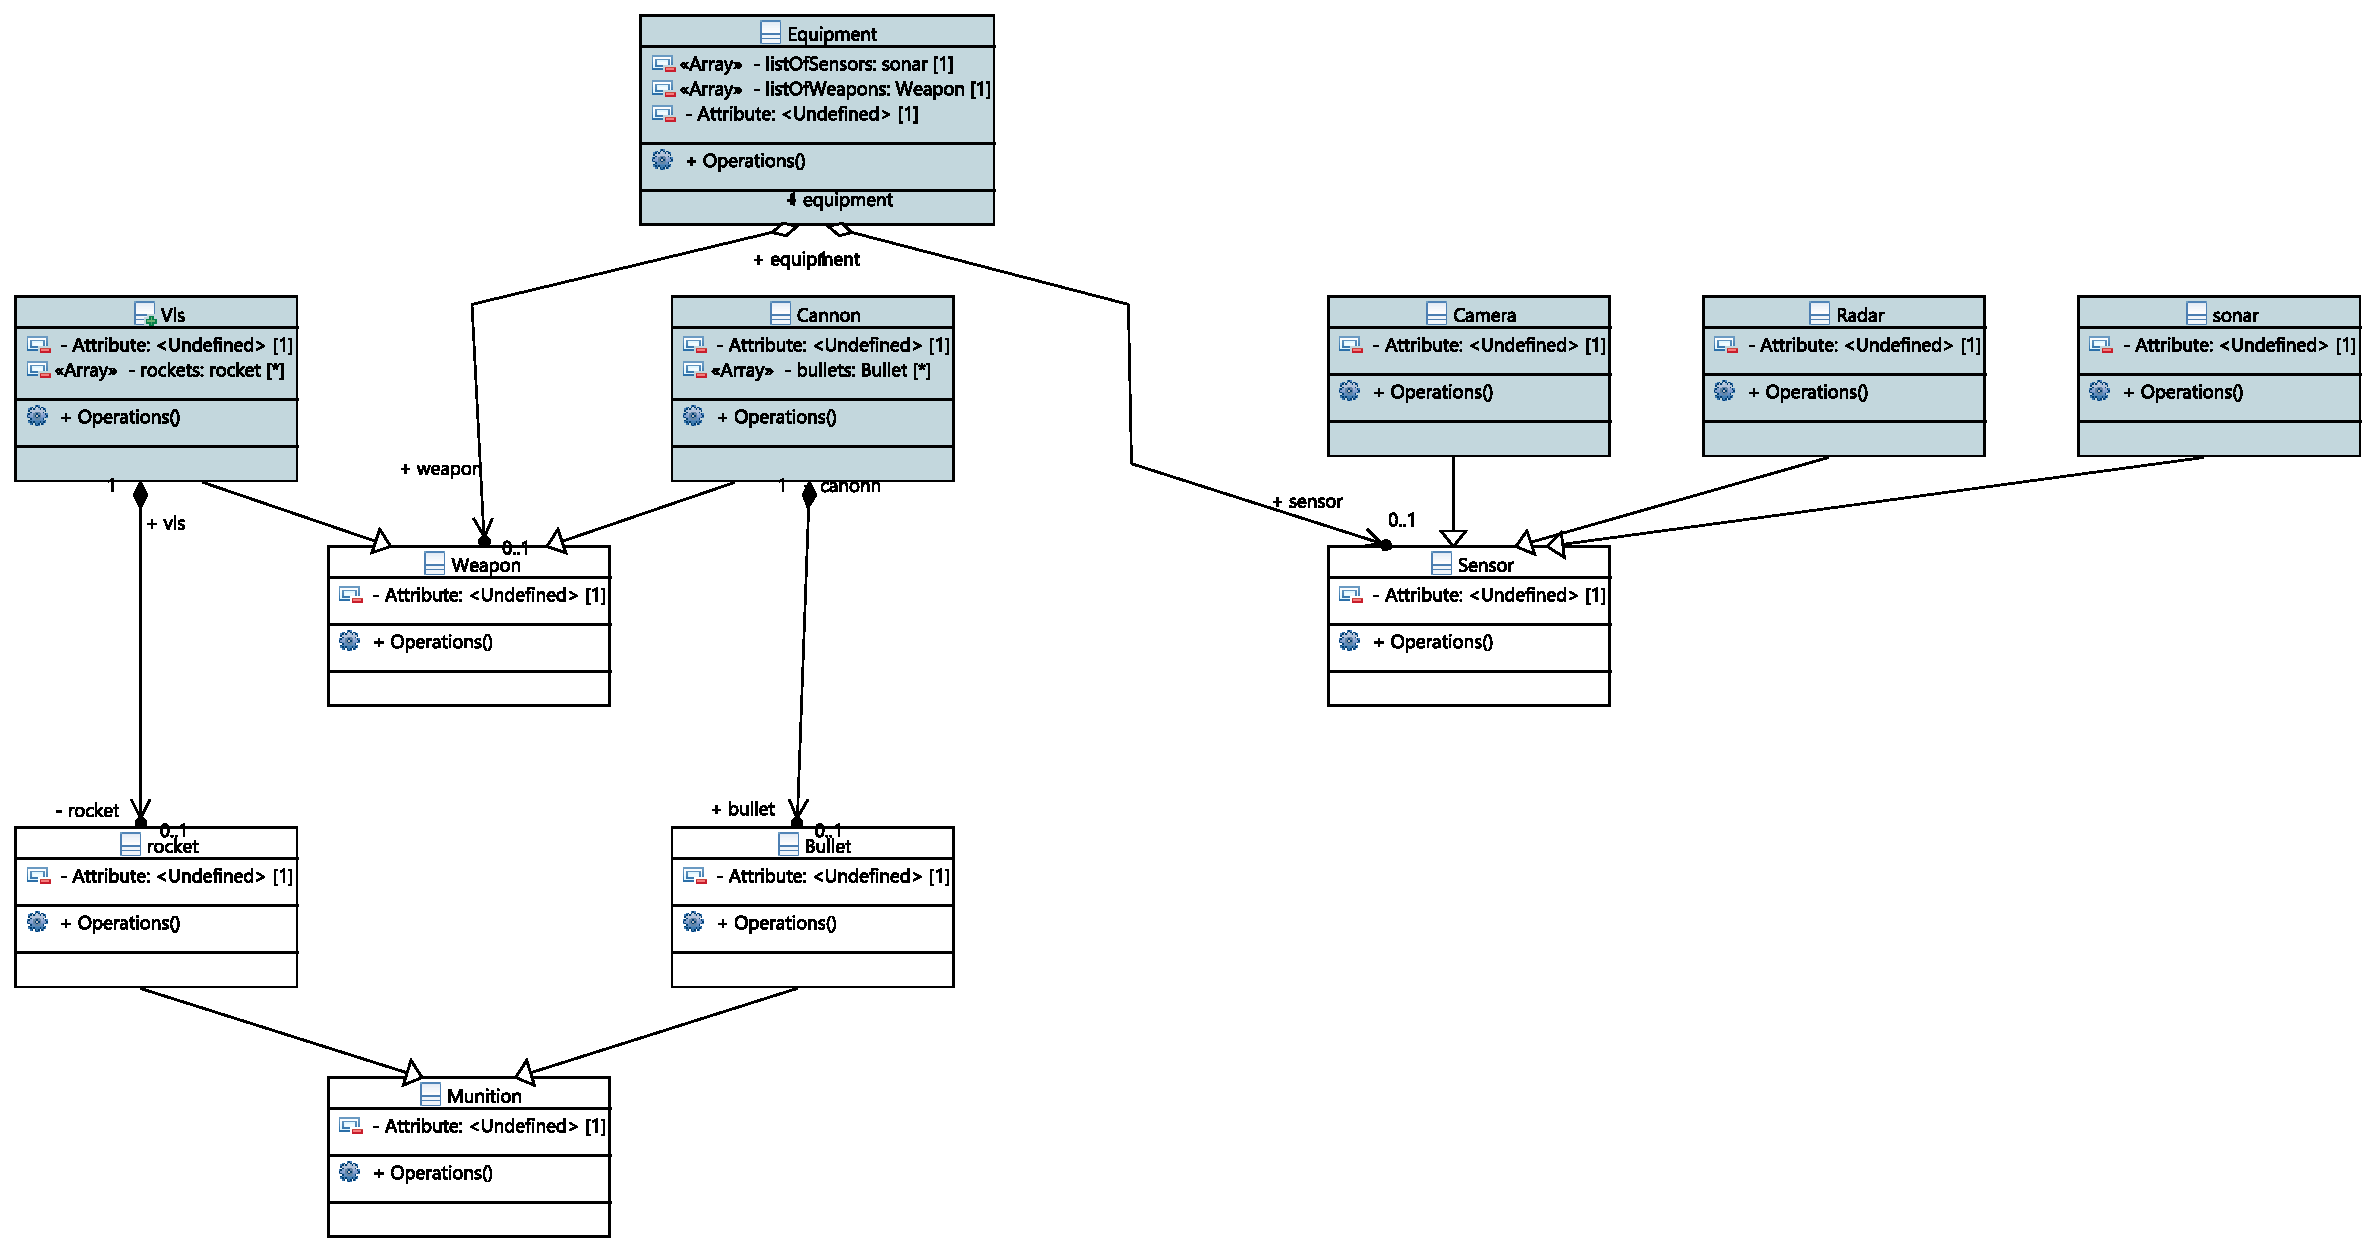
\includegraphics[height = 0.72\textheight,width =1.2\textwidth]{bilder/pdfvorlagen/equip}
			\caption[Ausrüstung]{Ausrüstung}
			\label{ausrüstung}
			% \end{minipage}
			%\end{minipage}
		}
	}
\end{figure}

%\begin{sidewaysfigure}[!h]
%	\centering
%	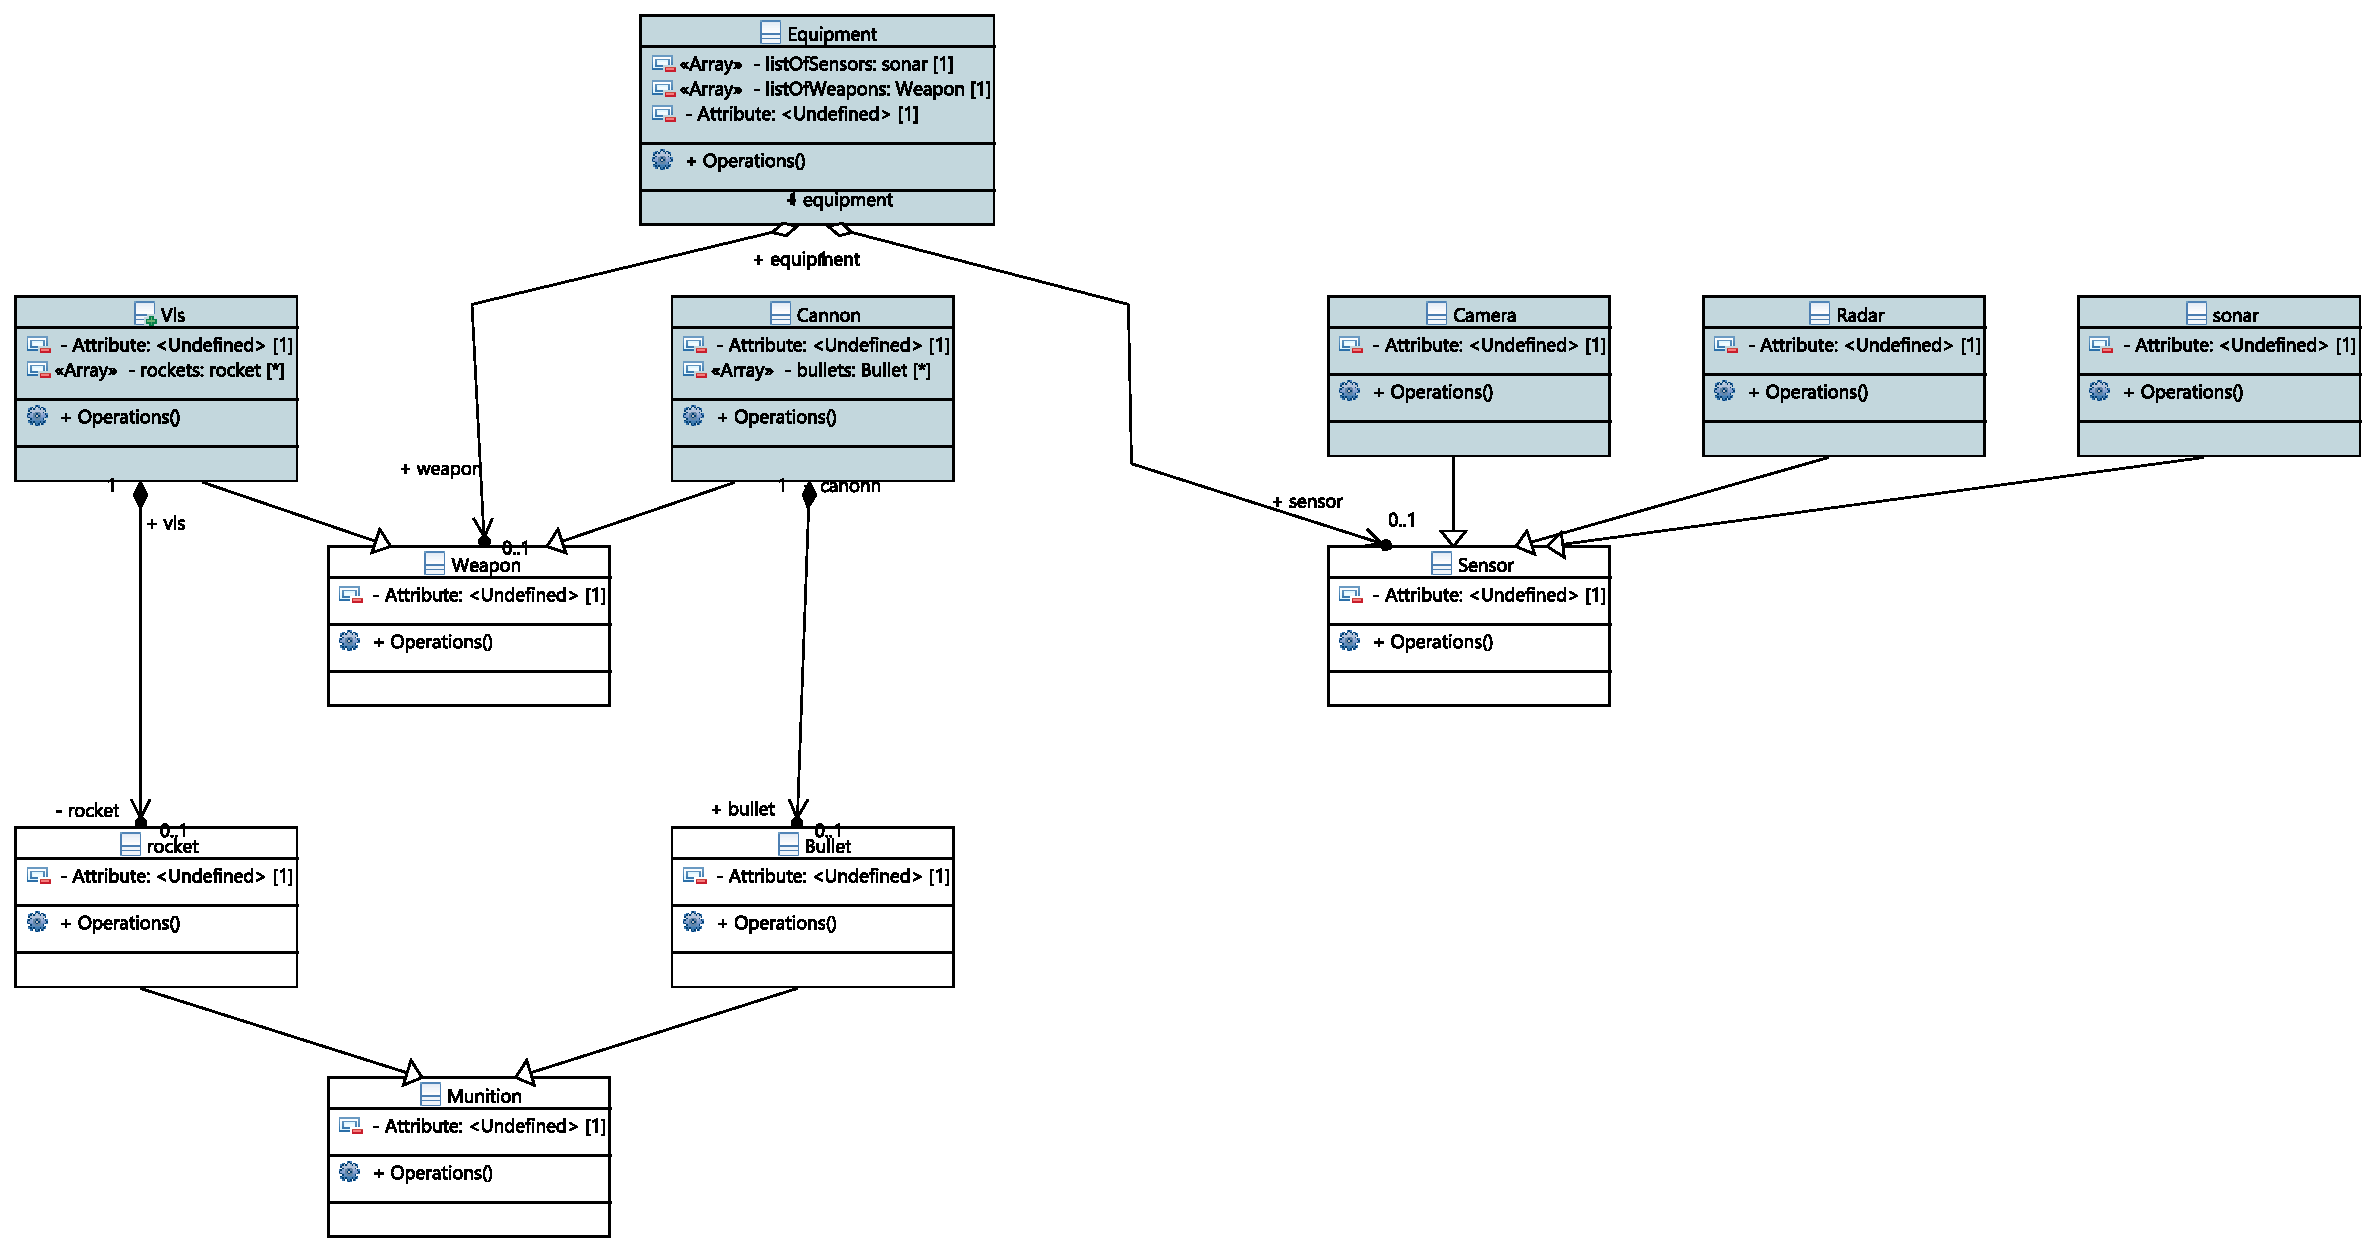
\includegraphics[height = 0.75\textheight,width =\textwidth]{bilder/pdfvorlagen/equip}
%	\caption[Ausrüstung]{Ausrüstung}
%	\label{ausrüstung}
%\end{sidewaysfigure}
